\section{序章}
\subsection{研究背景}
\label{1.1}
広島市で起きた平成30年7月の豪雨をはじめ
,土砂災害は全国各地で年間平均1099件(昭和57年から令和4年までの平均)
発生している\cite{mlit}.
土砂災害は発生前に
「降雨が続くにもかかわらず川の水位が低下する」や「崖から小石がパラパラと落ちる」
といった前兆現象が起こることが確認されている\cite{zentyou}.
そういった前兆現象を早期に検知し,住民に避難を促すことで
人的被害の削減につながると期待されている.本研究では,前兆現象の1つである
「降雨が続くにもかかわらず川の水位が低下する」現象に注目し,
この現象を捉えるため水位変動の推定を行う.

河川の水位変動を水位計を用いて計測する方法がある.しかし,
水位計にはコストの高さや整備の難しさといった問題があり,
そうした現状を踏まえ,安価で整備が容易な監視カメラを用いた水位推定が
水位計の代替案となっている\cite{seman}.
本研究では,河川の監視カメラ画像から水面領域を抽出し,水位の推定を行う.

\subsection{研究目的}
\label{1.2}
先行研究で渡邊\cite{watanabe}は,前兆現象の1つである「降雨が続くにもかかわらず川の水位が低下する」
現象に着目した.河川の様子を写した監視カメラ画像を4列×25枚の計100枚の
切抜画像へ変換を行い,それぞれの切抜画像に対して畳込みニューラルネットワークを使用し,
分類の際に出力される水面のソフトマックス値と元画像の縦座標値から算出する手法を
提案した.
しかし,訓練データと異なる日のテストデータに対しては
推定精度が低いという問題があった.

そこで,本研究でも同じ前兆現象に焦点を当て,深層学習を用いた
セマンティックセグメンテーションによる水面領域抽する手法(以下,SS手法)
を検討するために,その精度を評価した.また,深層学習を用いたセマンティックセグメンテーションでは,
一般的に訓練データとしてアノテーション付きの画像(以下,アノテーション画像)が多数
必要であり,アノテーション方法が精度に影響する.ただし,多数のアノテーション画像を手作業で作成するには過大な労力
がかかる.従って,可能な労力で必要な精度を達成するために,半自動的な作成方法を提案する.

\clearpage
%%%%%%%%%%%%%%%%%%%%%%%%%%%%%%%%%%%%%%%%%%%%%%
\section{関連研究}
%Nurの研究について
深層学習を用いたセマンティックセグメンテーションを使用して
河川の監視カメラ画像から水位推定を行った研究は存在している.
Nurら\cite{seman}は,河川の監視カメラ画像から水面領域を抽出するために
畳込みニューラルネットワークに基づくセマンティックセグメンテーションを提案した.
DeepLabv3+\cite{deeplabv3+}とSegNet\cite{segnet}という二つのセマンティックセグメンテーション
向け畳込みニューラルネットワークで作成した
モデルの領域抽出精度の比較を行った.結果はDeepLabv3+を用いて作成したモデル
の方が高精度で領域抽出できていることが確認された.
また,高い抽出精度を示したDeepLabv3+モデルを用いて,実際に,
5日間の水位推定と水位変動の観測を行った.推定した水位と実際の水位
は強い相関関係を示し,提案手法の有効性を報告した.

\clearpage
\subsection{DeepLabv3+}
\label{2.1}
DeepLabv3+\cite{deeplabv3+}はGoogle Research Teamによって考案されたセマンティックセグメンテーション
向け畳込みニューラルネットワークであり,旧バージョンのモデルから多くの改良が施された,最先端のモデルの一つである.
DeepLabv3+は図\ref{figure:DeepLabv3+}に示すようにエンコーダ・デコーダ構造を持ち,
Atrous convolutionとAtrous spatial pyramid poolingを備えている.

Atrous convolutionはAtrous rateというストライドに関するパラメータを持っており,
一般的な畳込み層より大きい受容野を持ち,効率的に畳込みすることが可能である.
また,それは式(1)のように表される.
式(1)の,$y[i]$は出力,$w[k]$は長さkのフィルタ,$x$は入力である特徴マップ,$r$はAtrous rate
を表す.

Atrous spatial pyramid poolingの特徴は,異なるAtrous rateで複数のAtrous convolution
を行い,それらを重ねアップサンプリングを行い,デコーダ部分で欠損した情報の復元に使用することである.
\begin{equation}
  \label{filter}
  \begin{center}
    $y[{i}]=\displaystyle\sum_{k}x[{i+r\cdot k}] \cdot w[{k}]$
  \end{center}
\end{equation}

\begin{figure}[ht] 
  \begin{center}
    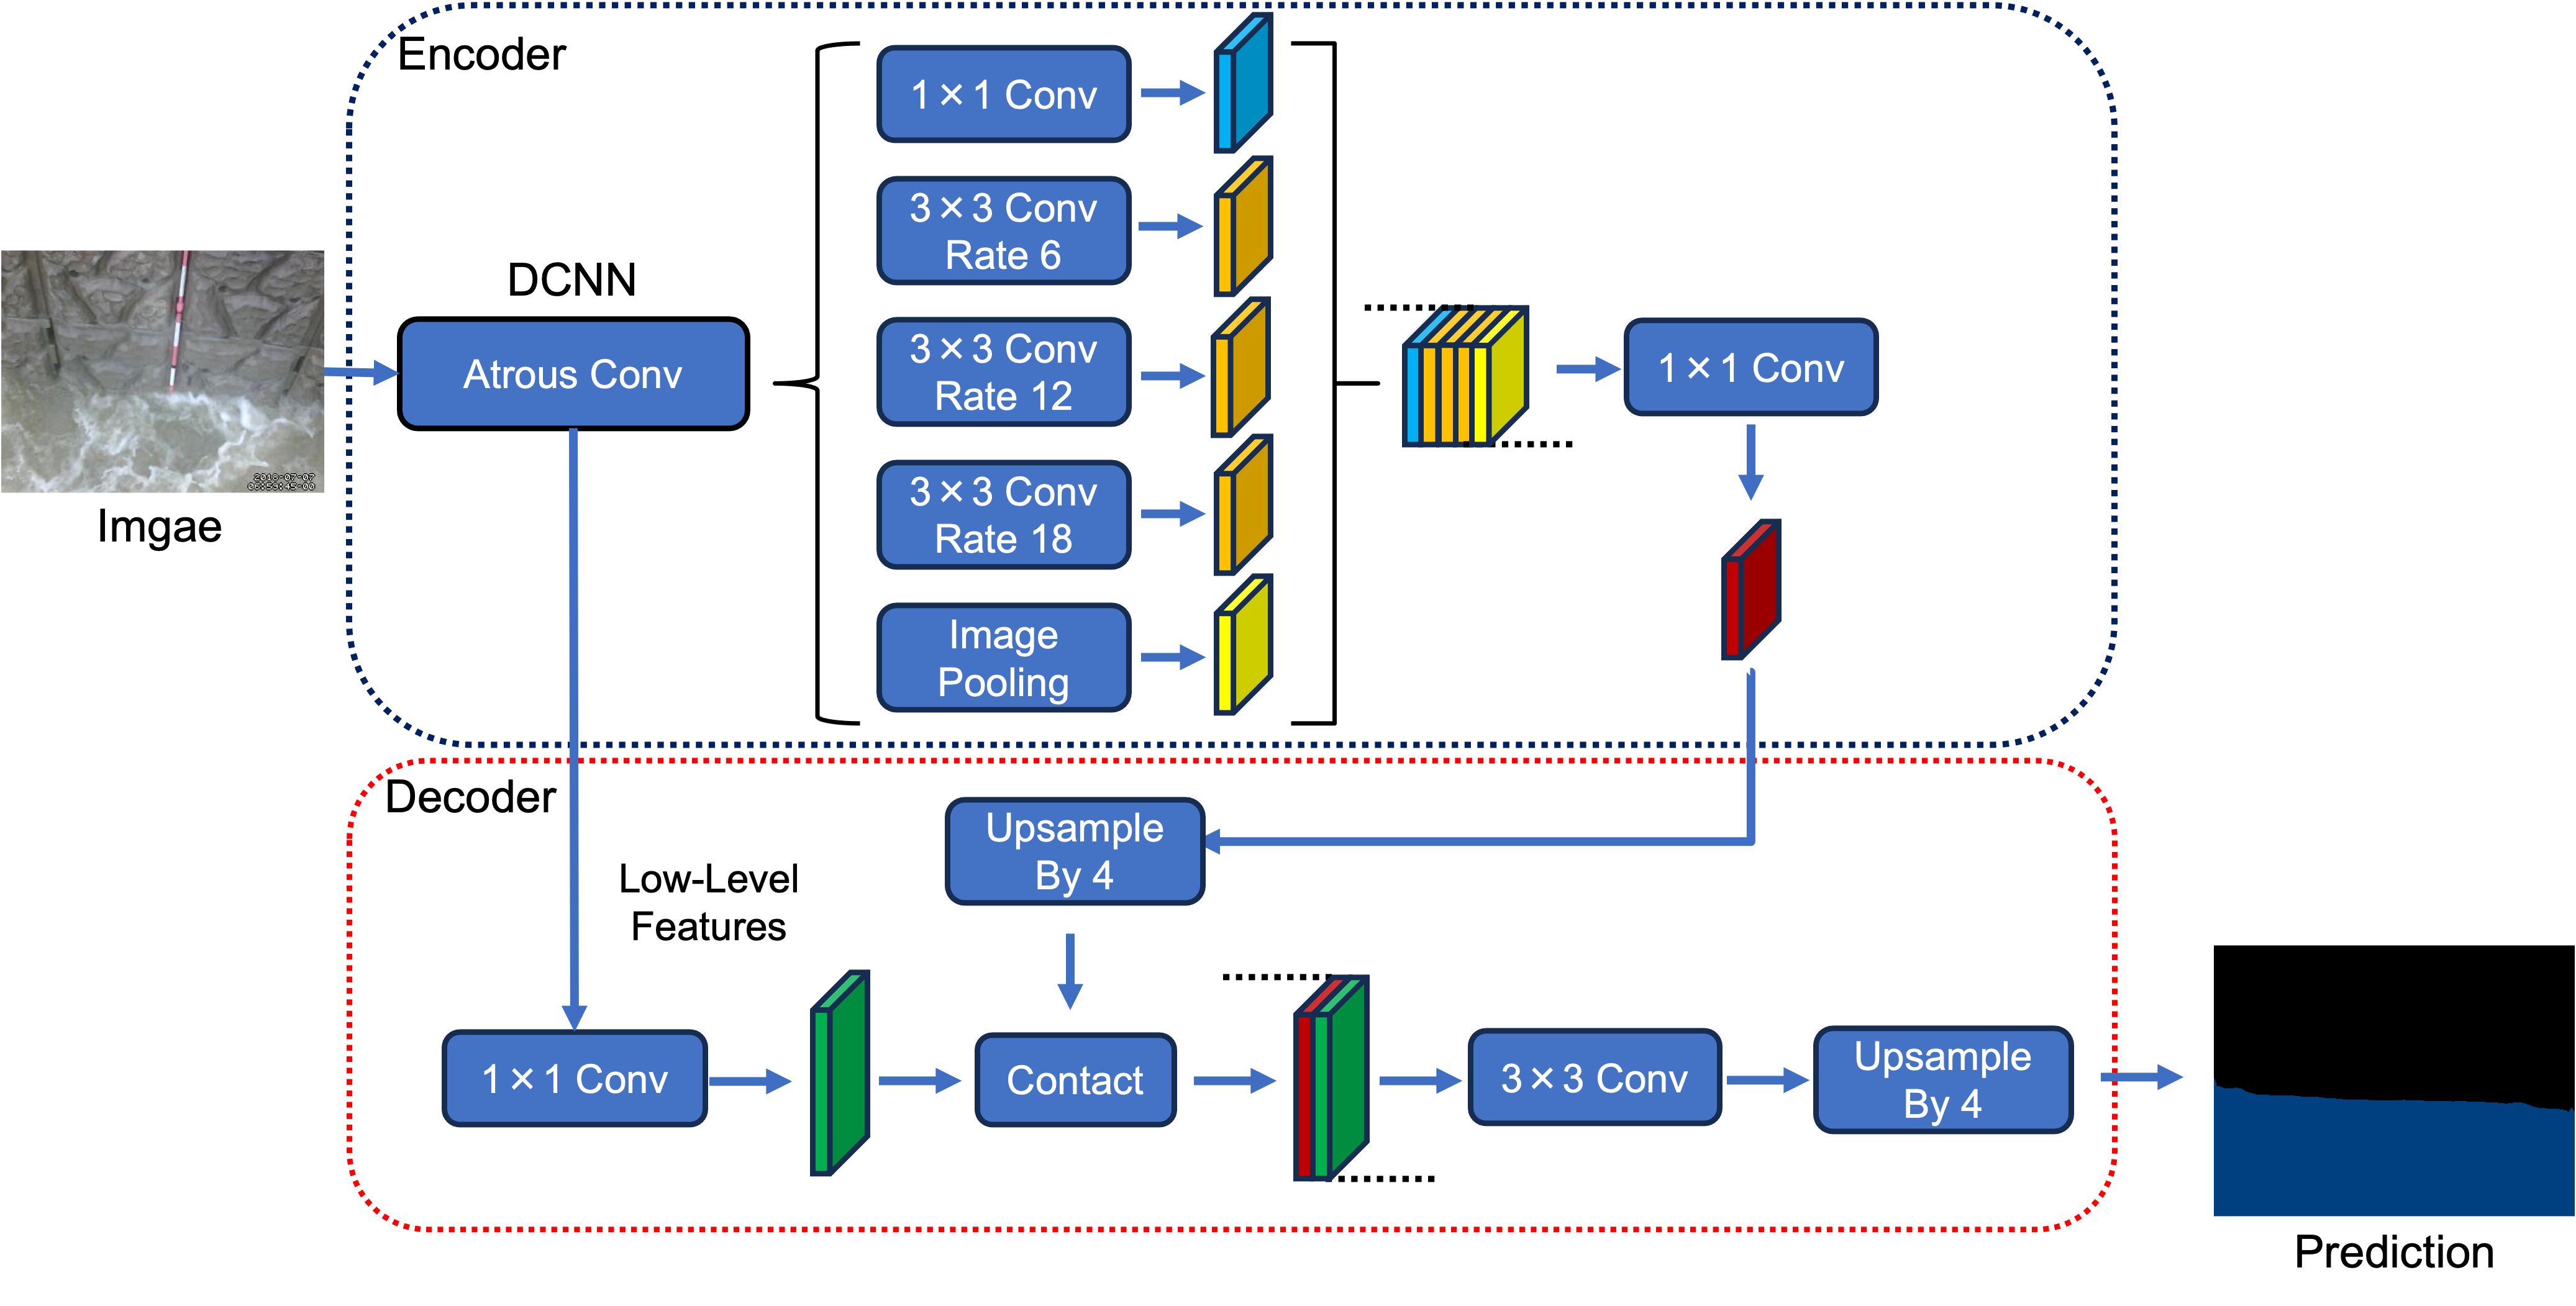
\includegraphics[width=\linewidth]{image/DeepLabv3+.png}
  \end{center}
  \caption{DeepLabv3+モデル}
  \label{figure:DeepLabv3+}
\end{figure}
\clearpage
%%%%%%%%%%%%%%%%%%%%%%%%%%%%%%%%%%%%%%%%%%%%%%
\section{先行研究}
\subsection{概要}
\label{3.1}
先行研究\cite{watanabe}は,土砂災害の前兆現象の一つである「降雨が続くにもかかわらず
川の水位が低下する」現象に着目した.河川の監視カメラ画像を図\ref{kirinuki}の
ように切り抜き,切抜画像が水面かどうかを畳込みニューラルネットワークによって
判別を行い,判別されるときに出力される水面クラスのソフトマックス値と画像の縦座標値を用いて
水位の変動を推定した.深層学習を用いて推定した水位変動と実際の水位変動
との相関を評価をした.

\subsection{画像の切り抜きとラベル付け}
\label{3.2}
河川の監視カメラ画像の幅を5等分(幅64高さ×240pixel)になるよう
に切り分け,そのうち,水位計測ポールを含む
中央の列を除外を行った.残った各4列に対して,
高さを元の河川画像を5等分した大きさ(各48pixel)となるように,幅64×
高さ48pixelの画像を縦に8pixelずつ移動させて,最下段まで切り抜きを行った.
切り抜いた画像に対して,以下に示す3つのクラスに分類してラベル付けを行った.
\begin{description}
    \item・ 「水面」  : 水面が写っている画像
    \vspace{-2mm}
    \item・ 「壁面」  : 壁面が写っている画像
    \vspace{-2mm}
    \item・ 「その他」 : 水面と壁面の両方が含まれる画像
\end{description}

\vspace{2mm}
\begin{figure}[h] 
  \begin{center}
    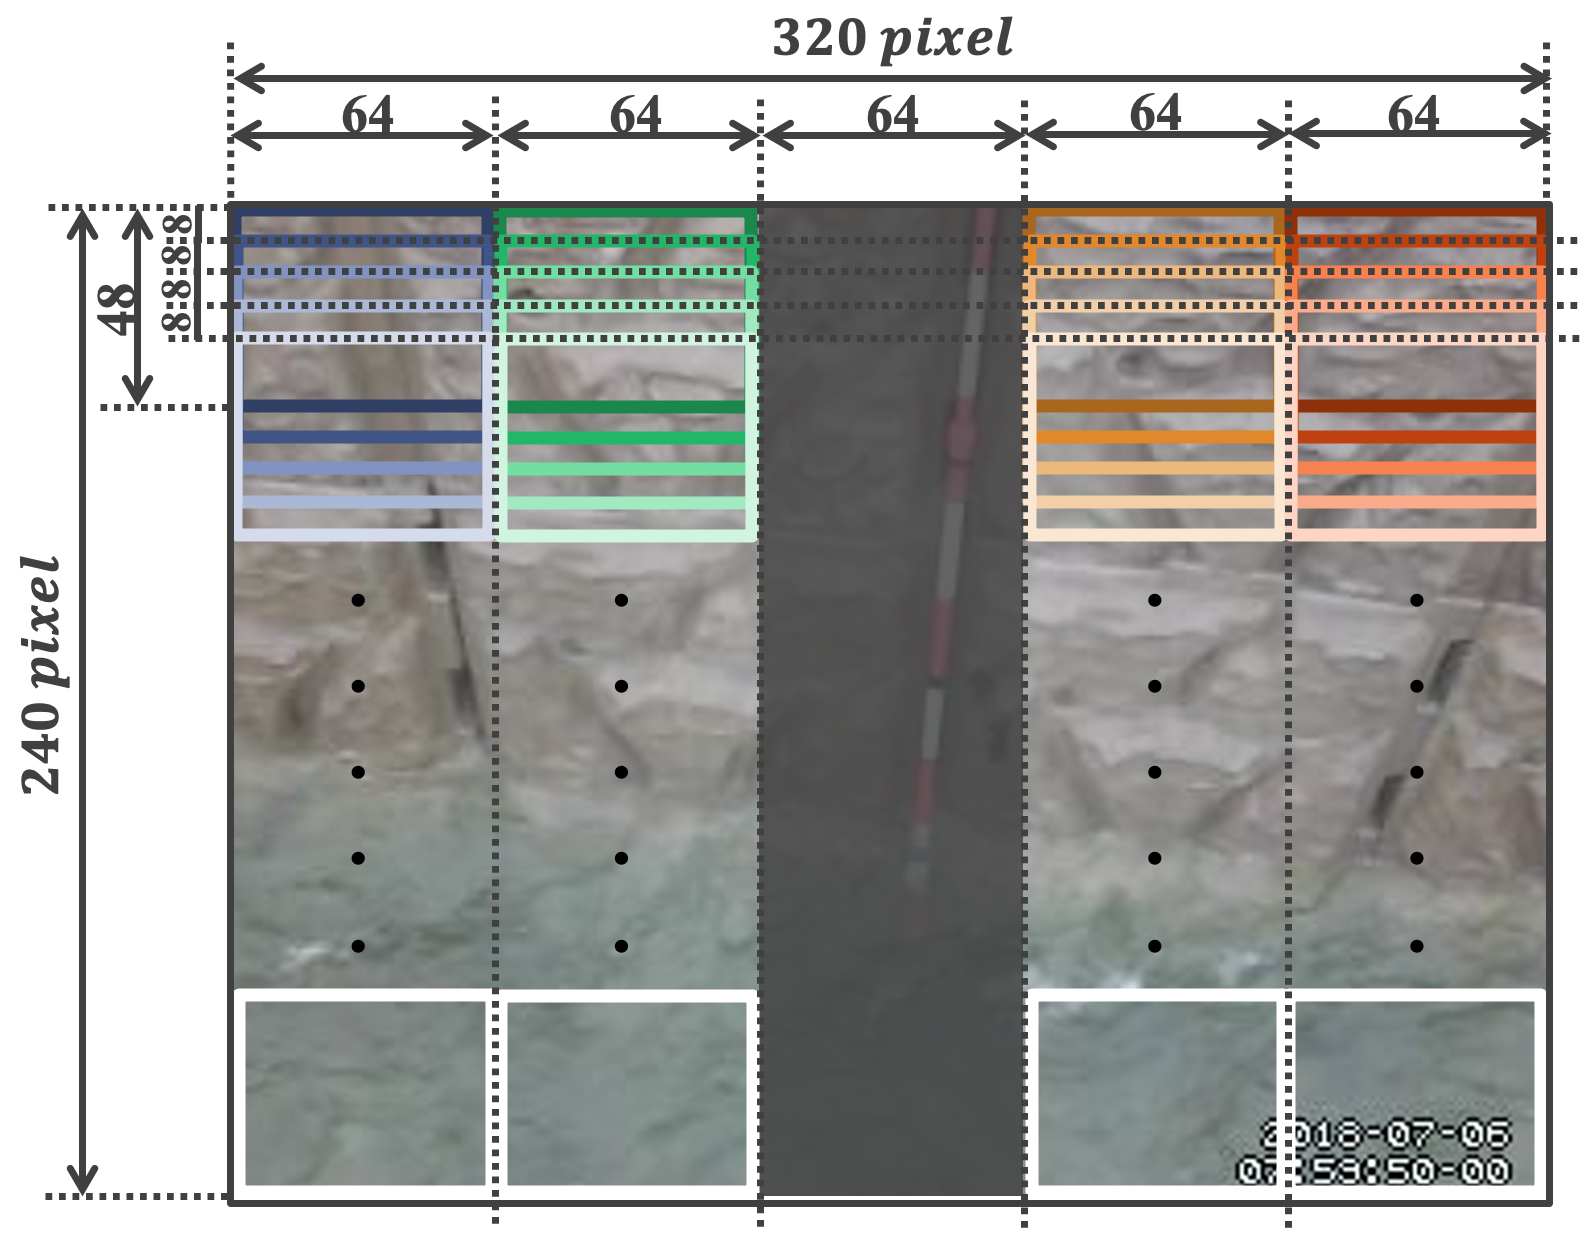
\includegraphics[width=90mm]{figs/kirinuki.png}
  \end{center}
  \caption{切抜画像の生成}
  \label{kirinuki}
\end{figure}

\clearpage
  
\label{3.3}
\subsection{水位の推定方法}
\ref{3.2}節で生成した切り抜き画像を用いて,河川の水位を推定する.各切抜画像に対して
,畳込みニューラルネットワークで学習と分類を行った際に,出力される水面クラスの
ソフトマックス値$S_{water}$と,元画像における縦の座標値$y$を用いて水位の推定を行った.
水位の推定値$E$は元画像から$n$枚の切抜画像が得られたとき以下の式(\ref{e_1})で導出した.
\vspace{5mm}
\begin{equation}
  \label{e_1}
  E=\frac{\sum_{n} y S_{water}}{\sum_{n} S_{water}}
\end{equation}
\vspace{3mm}

例として,水位の推定値を算出する流れを図\ref{suii}で説明する.なお,
説明の際はわかりやすいように,簡略した5列×5枚で切り抜いた場合
について考える.まず,中央の列は測定ポールを含んでいるため除外する.
続いて,各切抜画像を分類し,水面クラスに属する確率に相当する,
ソフトマックス値を算出する(切抜画像内の数値).
また,元の河川の画像における,各切抜画像の上辺と下辺の高さを二分する高さの座標値を求める.
最後に,式(\ref{e_1})に数値を代入することで水位の推定値を算出する.
例の場合,水位の推定値 E = 190.8である.このとき,
壁面と水面の境界線は図\ref{suii}の白線の部分であるが,水位の推定値は,
画像中における水面の面積の半分にする縦の座標値に相当する.
例で求めた水位の推定値にしたがって,縦の座標値波線の矢印を引くと,
水面の面積をおよそ半分にする位置に求まっていることがわかる.
\vspace{3mm}
\begin{figure}[h] 
  \begin{center}
    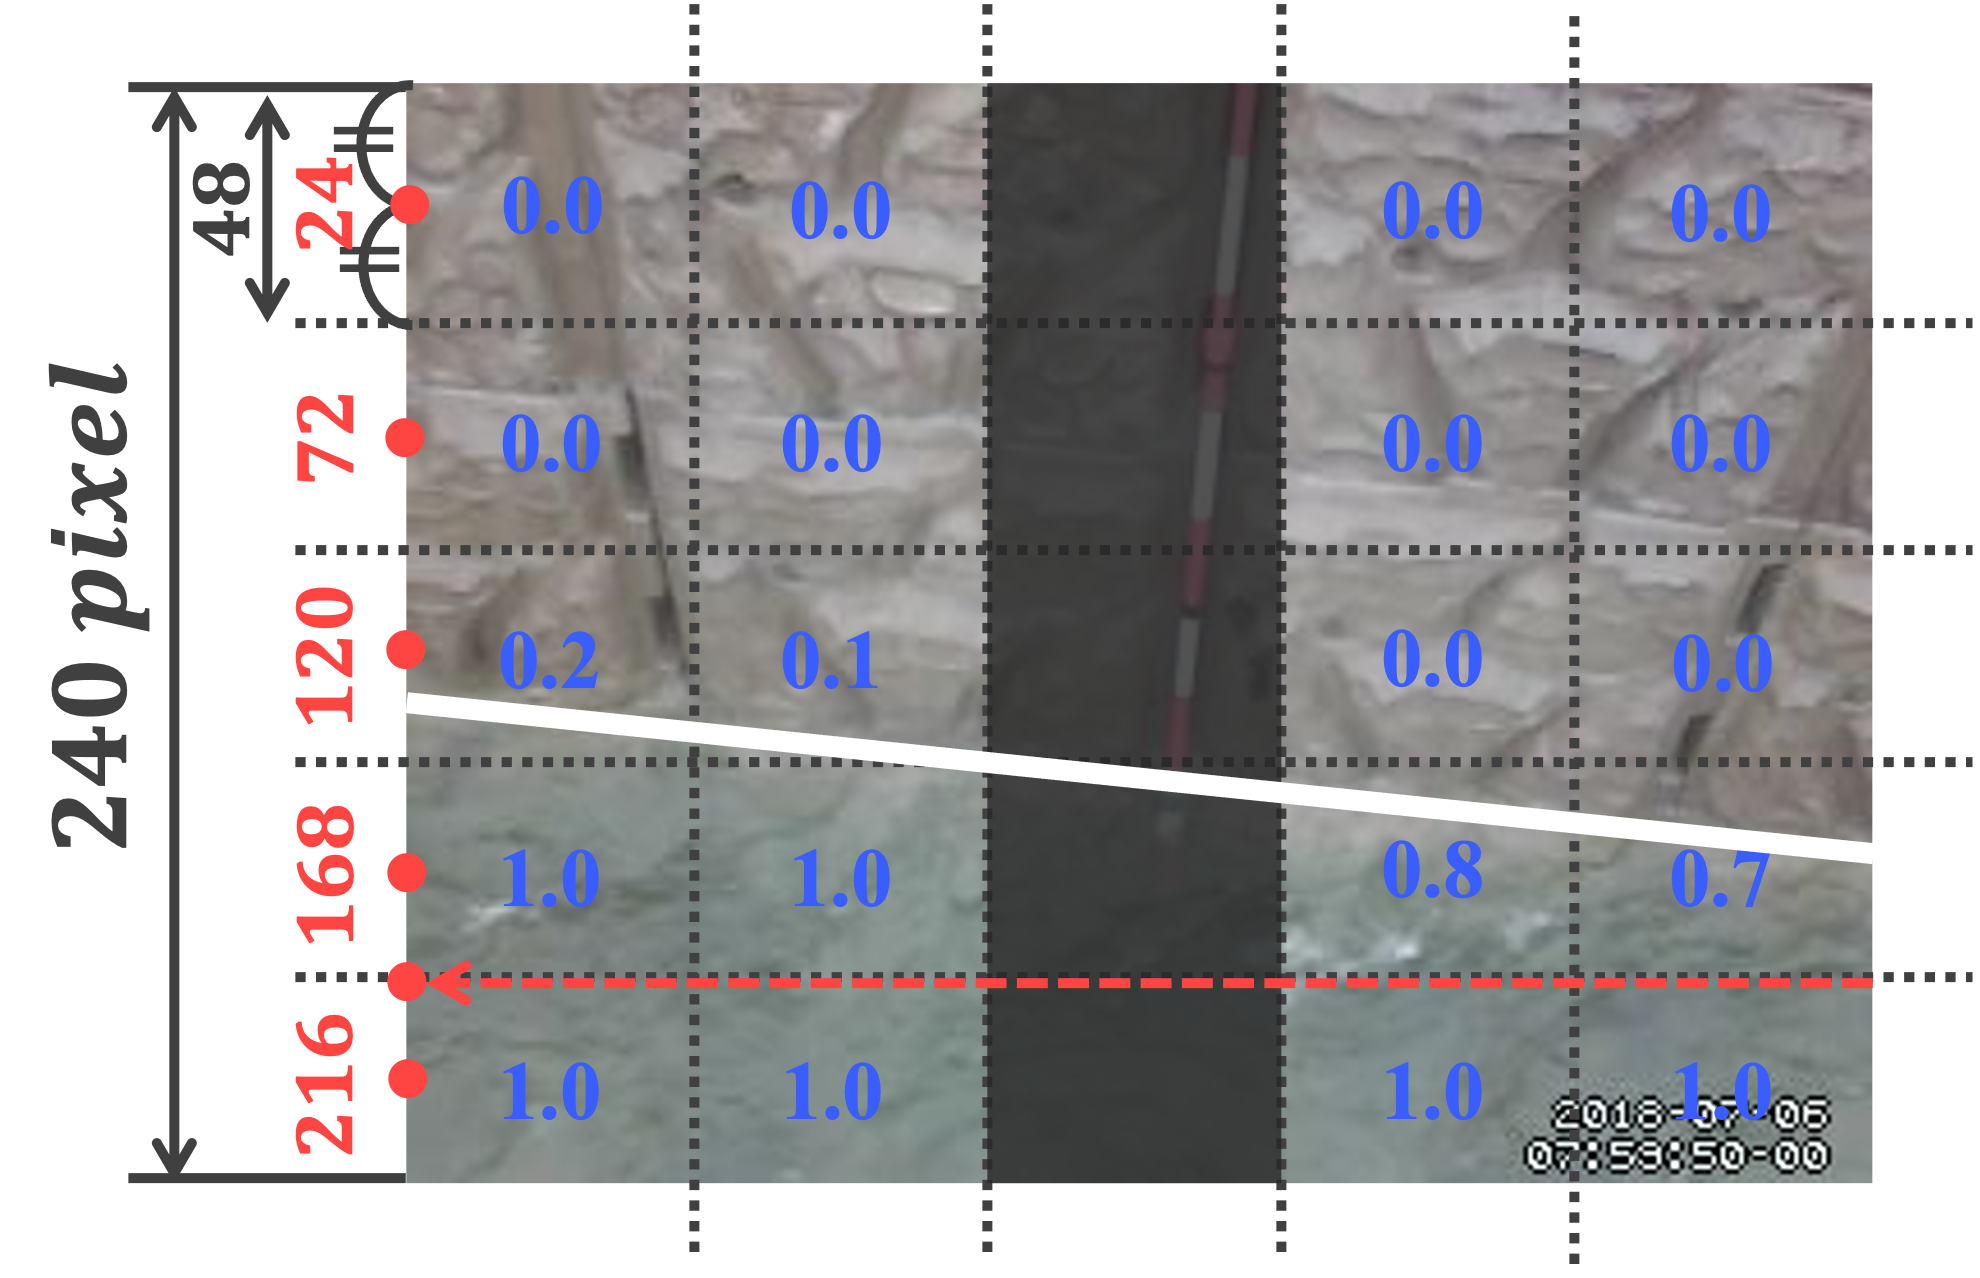
\includegraphics[width=100mm]{figs/suii.png}
    \end{center}
    \caption{推定値算出の流れ}
    \label{suii}
\end{figure}

\clearpage
\subsection{相関係数による評価}
\label{3.4}
式\ref{e_1}によって推定された推定値$E$と,水位計測ポールを参考にして
10分ごとに目視で測定した水位を線形補完した値(測定値)との相関係数を用いて評価した.
\vspace{5mm}
\begin{table}[ht]
  \centering
  \caption{推定値と測定値の相関}  
  \begin{tabular}{rr} \bhline{1.5pt}
     クラス&相関係数 \\ \hline 
   2分類&  0.956\\ \hline
   3分類&  0.930\\ \hline    
  \end{tabular}
  \label{tb:sokan1}
\end{table}
\vspace{5mm}

なお,「水面」「壁面」の2つのクラスで学習と分類を行った
結果を2分類,「水面」「壁面」「その他」の3つのクラスで学習
と分類を行った結果を3分類とした.
\clearpage

%%%%%%%%%%%%%%%%%%%%%%%%%%%%%%%%%%%%%%%%%%%%%%
\section{提案手法}
\subsection{概要}
\label{4.1}
深層学習を用いたセマンティックセグメンテーションでは,
一般的に訓練データとしてアノテーション画像が多数必要であり,アノテーション方法が
精度に影響する.
また,アノテーション画像を手作業で作成する場合,過大な労力がかかる.そこで,本研究では,
可能な労力で必要な精度を達成するための,半自動的なアノテーション方法を提案する.
図\ref{images}に使用した元画像とアノテーション画像の例を示す.

画像内の水面領域の面積割合は水位が上昇するとともに大きくなるため,
水面領域の面積割合から水位へ変換する式を作成した.SS手法を用いて領域抽出を
行った画像から,変換式を用いて水位の推定を行った.

\vspace{10mm}

\begin{figure}[ht] 
  \begin{center}
    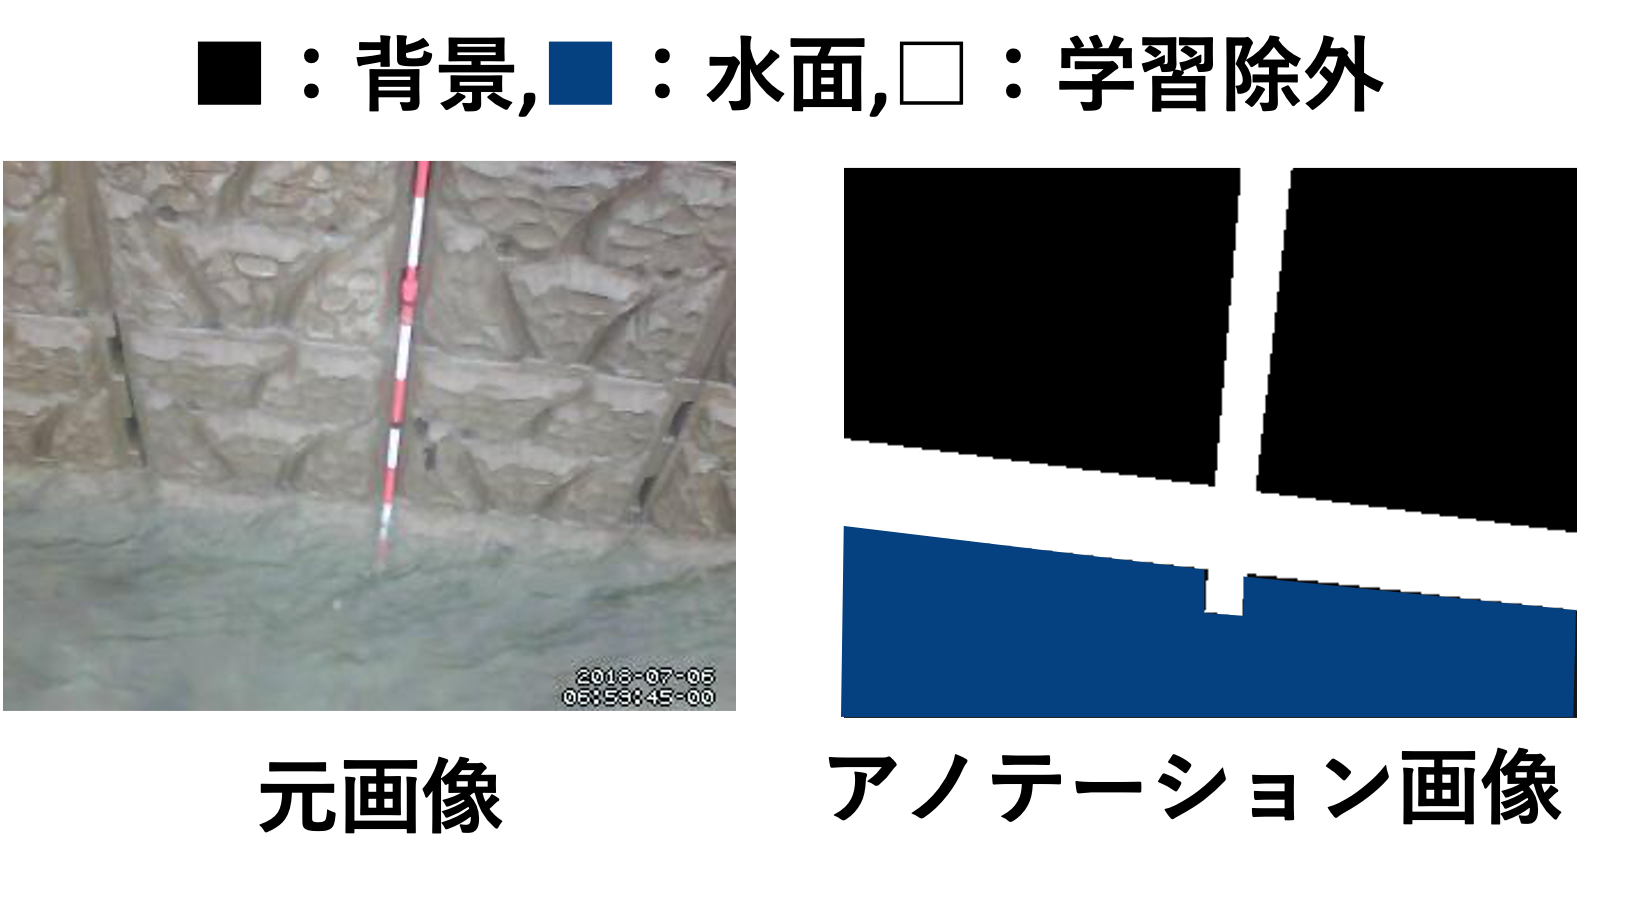
\includegraphics[width=\linewidth]{image/images.png}
  \end{center}
  \vspace{-3mm}
  \caption{元画像とアノテーション画像の例}
  \label{images}
\end{figure}
\clearpage

\subsection{アノテーション方法}
\label{4.2}
本研究で扱った河川の監視カメラ画像には「水面」「壁面」「水位計測ポール」「撮影日時」
の4つの範囲がある.従って,本研究では以下の方法によってアノテーション画像を
作成した.
\begin{description}
  \item・「水面」と「壁面」の範囲は水位によって変化するため,まず目視
  によって10分毎の水位を推定し,その測定値から線形補間によって自動的に範囲を
  決定した.
  \vspace{-3mm}
  \item・確実なラベル付けを行うため,「水面」と「壁面」の境界が曖昧な
  範囲は,学習対象から除外した.
  \vspace{-3mm}
  \item・「水位計測ポール」と「撮影日時」の範囲は時間によらず変化しないため,目視で
  決定した.
  \vspace{-3mm}
\end{description}
「水面」と「壁面」の範囲決定の様子を図\ref{ano2}に示す.
\vspace{20mm}
\begin{figure}[ht]
  \centering
  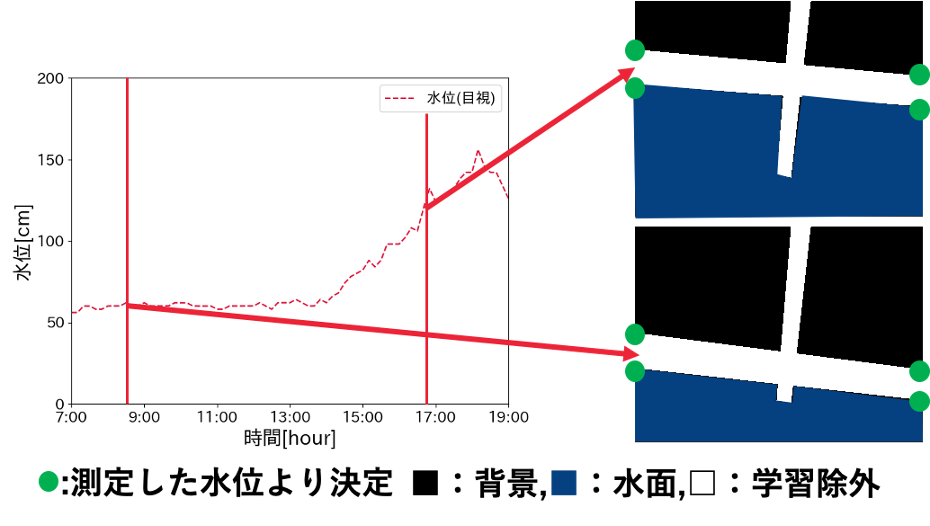
\includegraphics[keepaspectratio,width=\linewidth]{image/ano2.png}
  \caption{範囲決定の流れ}
  \label{ano2}
\end{figure}
\clearpage

\subsection{水位の推定方法}
\label{4.3}
画像内の水面領域の面積割合と水位の散布図を図\ref{soukan}に示す.
また,水面領域の面積割合と水位の相関係数は0.99となった.
従って,水面領域の面積割合から水位へ値を変換する式を作成した.
この変換式を使用して,領域抽出結果画像から水位の推定を行った.
\vspace{5mm}
\begin{figure}[h] 
  \begin{center}
    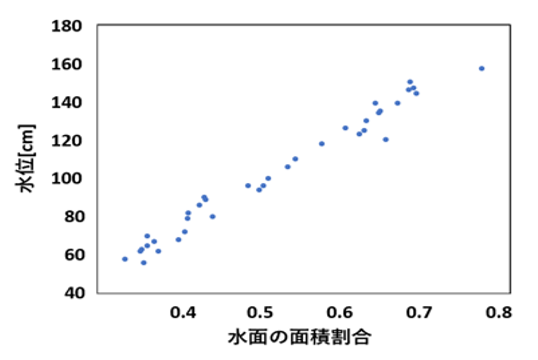
\includegraphics[width=0.8\linewidth]{image/soukan.png}
  \end{center}
  \caption{水面領域の面積割合と水位の散布図}
  \label{soukan}
\end{figure}
\clearpage
%%%%%%%%%%%%%%%%%%%%%%%%%%%%%%%%%%%%%%%%%%%%%%
\section{評価実験}
目視で計測した水位とSS手法を用いて推定した水位のRMSE(Root Mean Square Error)
を先行研究\cite{watanabe}で比較することで,SS手法の評価を行う.
また,提案したアノテーション方法で作成したモデルの領域抽出精度を評価することで
提案手法の有効性を示す.

本研究では河川画像として,本学情報工学科モニタリングネットワーク研究室にて
運用中の広島市安佐北区三入地区桐原川の監視システムにおいて撮影された
図\ref{togegawa}の監視カメラ画像を使用した.
また,畳込みニューラルネットワークによるセマンティックセグメンテーションのシステムとして,
DeepLabv3+\cite{deeplabv3+}を用いた.

\vspace{20mm}
\begin{figure}[h] 
  \begin{center}
    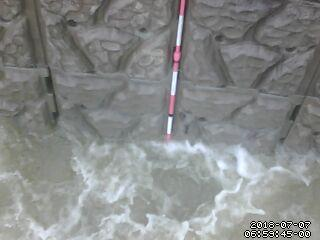
\includegraphics[width=130mm]{image/070001.jpg}
  \end{center}
  \caption{桐原川の監視カメラ画像}
  \label{togegawa}
\end{figure}
\clearpage

\subsection{学習モデルの構築と評価}
\label{5.1}
セマンティックセグメンテーションモデルの
学習回数を変化させて領域抽出を行い,IoU(Interaction over Union)\cite{IoU}
を評価することでモデルの適切な学習回数の調査を行った.

領域抽出結果についての評価は,Mean IoUを用いて行われるのが一般的である.IoUは式(\ref{IoU})
で表せられる予測領域と正解領域のオーバーラップ率を意味する値である.式(\ref{IoU})を構成するTP,FP,FNの定義は図
\ref{tp}に示す.
すべての画像に対するIoUをクラス毎に平均したAverage IoUを,さらに全クラスで平均した値がMean IoUとなる.
ただし,本研究ではクラス数が少なく,水面クラスの抽出結果に対してのみ評価を行うことを目的としているため,水面クラスの
Average IoU(以下,IoU)に着目して評価を行うこととした.

\begin{equation}
  \label{IoU}
  \mbox{IoU} =  \frac{\mbox{TP}}{(\mbox{TP}+\mbox{FP}+\mbox{FN})}
\end{equation}
\vspace{5mm}
\begin{figure}[ht] 
  \begin{center}
    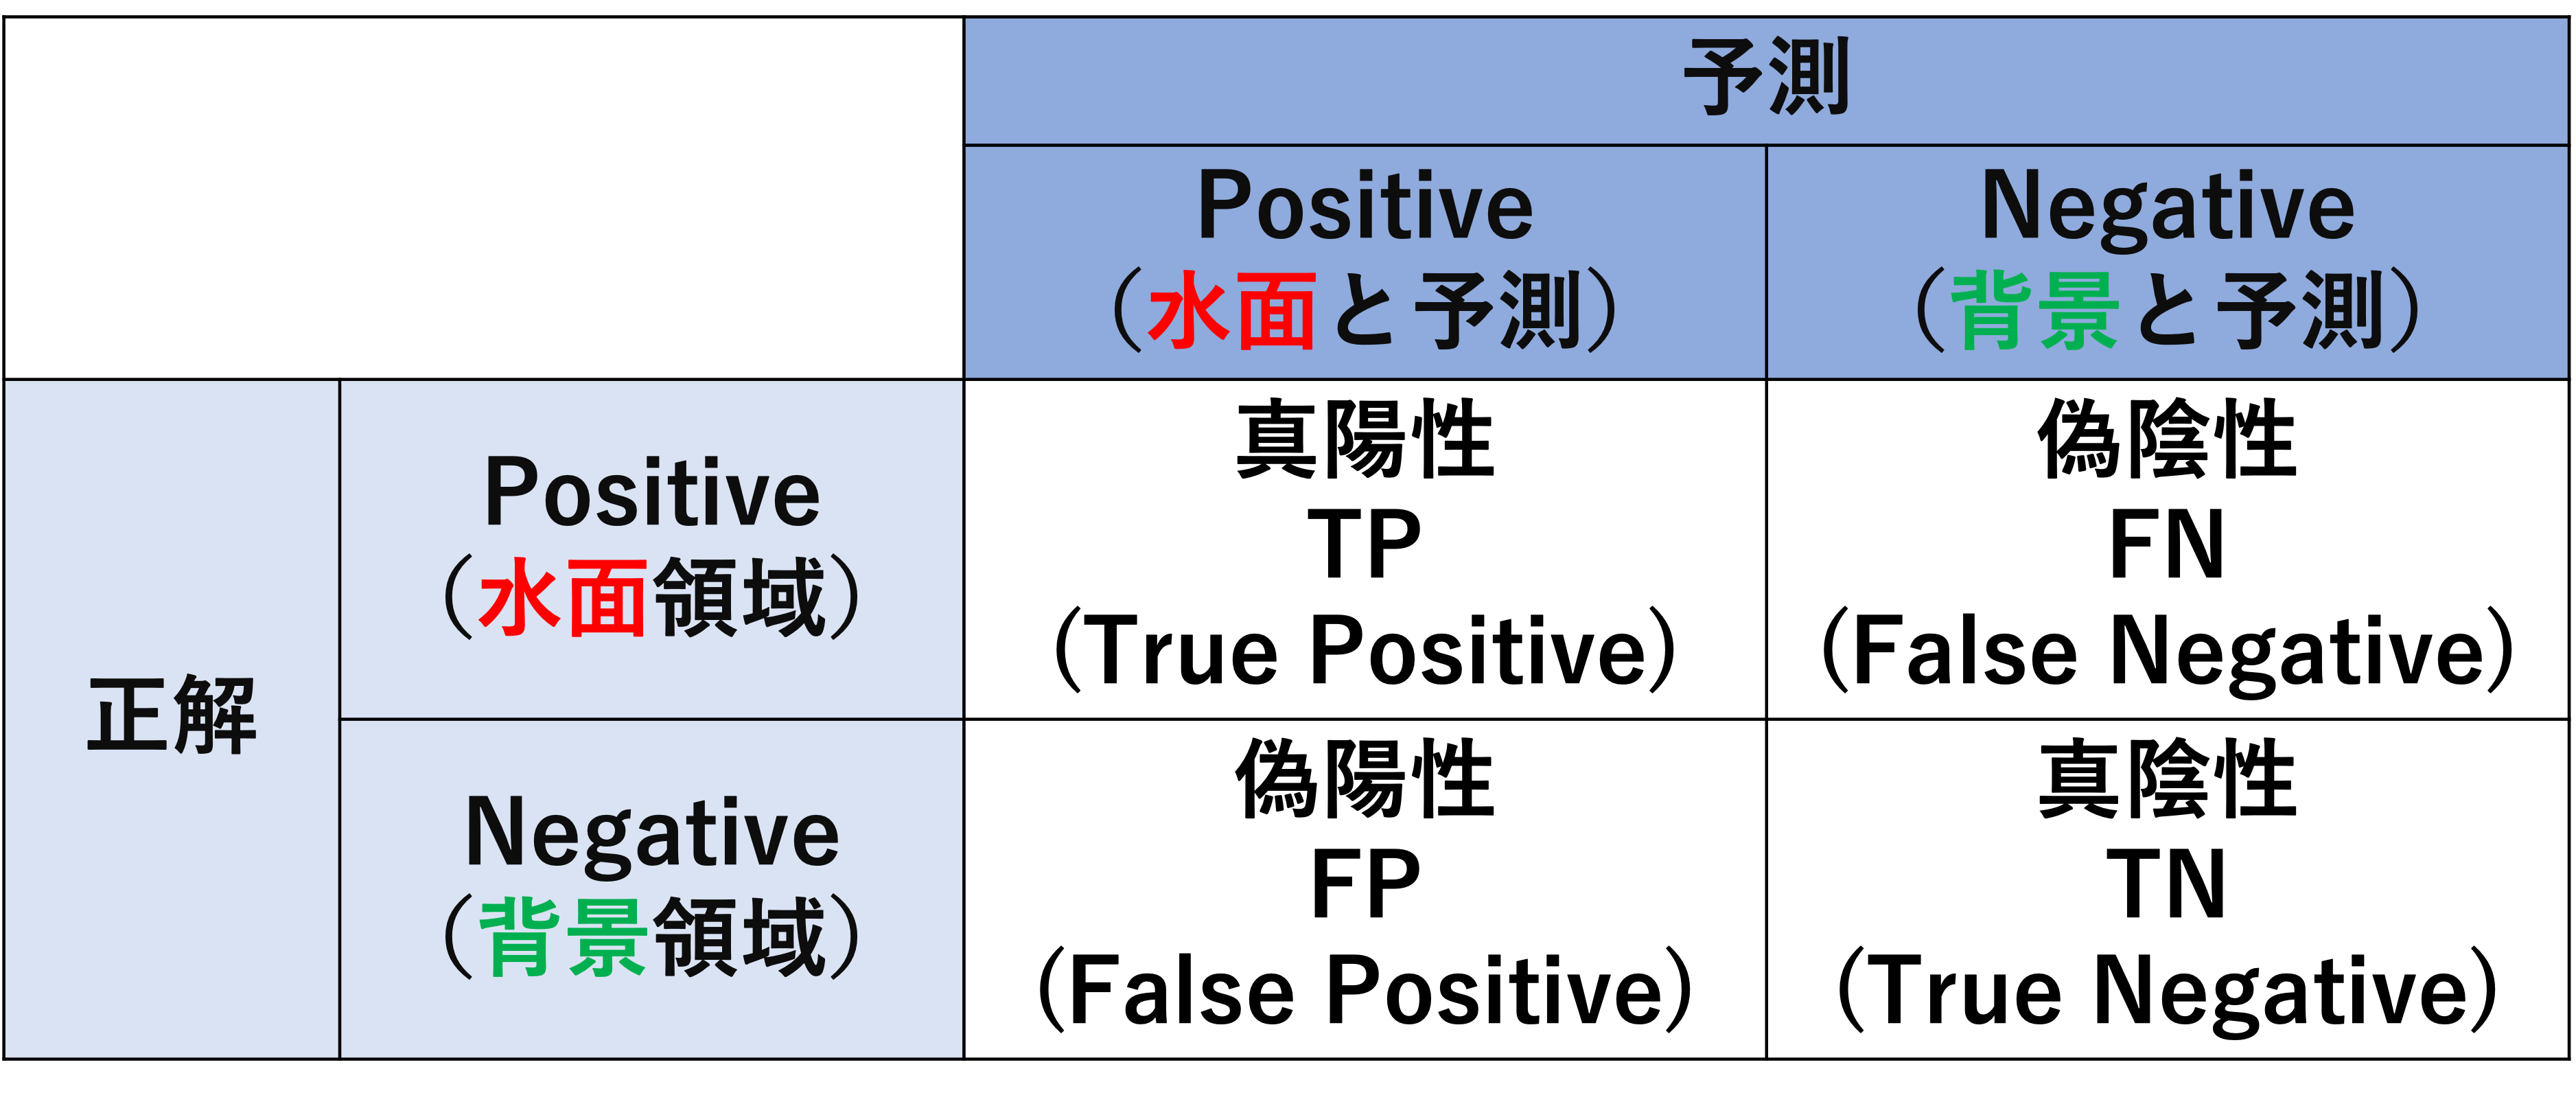
\includegraphics[width=150mm]{image/TP.png}
  \end{center}
  \caption{領域抽出における分類問題の混合行列の定義}
  \label{tp}
\end{figure}

\vspace{5mm}
2018年7月6日の7:00から19:00までの画像を訓練データ(8147枚)に,
テストデータには同年の7月7日同時間帯の画像データ(8086枚)を用いた.
また,モデル作成に使用したアノテーション画像は以下に示す設定(設定A)でアノテーションした.

\begin{description}
    \item・ 「水面」      : 水面ラベル
    \vspace{-2mm}
    \item・ 「壁面」      : 背景ラベル
    \vspace{-2mm}
    \item・ 「水位計測ポール」 : 学習除外ラベル
    \vspace{-2mm}
    \item・ 「撮影日時」    : 水面ラベル
\end{description}
\clearpage

学習回数を50,100,200,300...1000と変化させてセマンティックセグメンテーションモデル
セマンティックセグメンテーションモデルを作成した.
作成したモデルを用いて領域抽出を行い,IoUを求めた.
図\ref{figure:learn}はモデルの学習回数とIoUの関係を表した
グラフである.

\begin{figure}[ht] 
  \begin{center}
    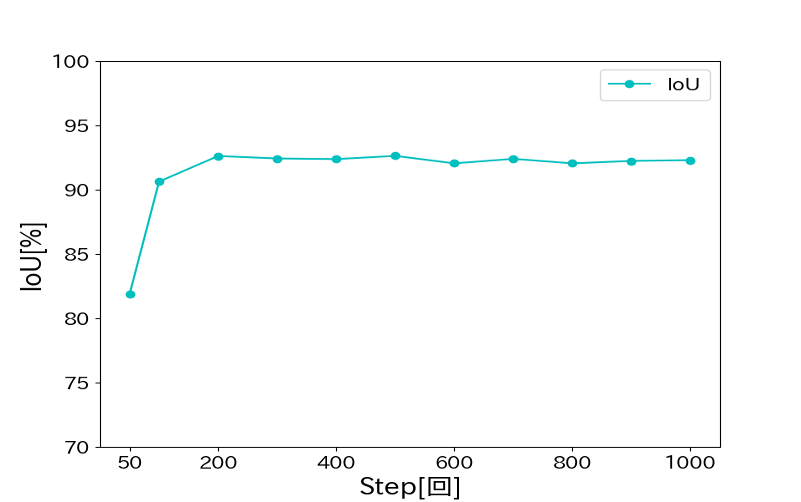
\includegraphics[width=150mm]{image/learn.png}
  \end{center}
  \caption{学習回数とIoUの関係}
  \label{figure:learn}
\end{figure}

\subsection{先行研究との比較}
\label{5.2}
SS手法の領域抽出精度を評価するため,時系列の河川の監視カメラ画像に
先行研究\cite{watanabe}の手法とSS手法を適応し,推定した水位と目視で計測した水位とのRMSEを比較した.
先行研究のラベル設定と統一するため,設定Aでアノテーションを行い,
訓練データには7月6日の画像を,テストデータには7月6日と7月7日の画像を使用した.

SS手法と先行研究の手法に対し,
水位を推定したとき,測定値とのRMSEは表\ref{senkou_ss}の通りとなった.
また,測定値と比較した結果を図\ref{ss_0706}から図\ref{senkou_0707}に示す.

\vspace{5mm}
\begin{table}[ht]
  \centering
  \caption{推定値と測定値のRMSE(cm)}  
  \begin{tabular}{lrr} \bhline{1.5pt}
     &7月6日&7月7日 \\ \hline 
   SS手法&8.05&  15.02\\ \hline  
   先行研究&26.00&  163.44\\ \hline  
  \end{tabular}
  \label{senkou_ss}
\end{table}


\begin{figure}[h] 
  \begin{center}
    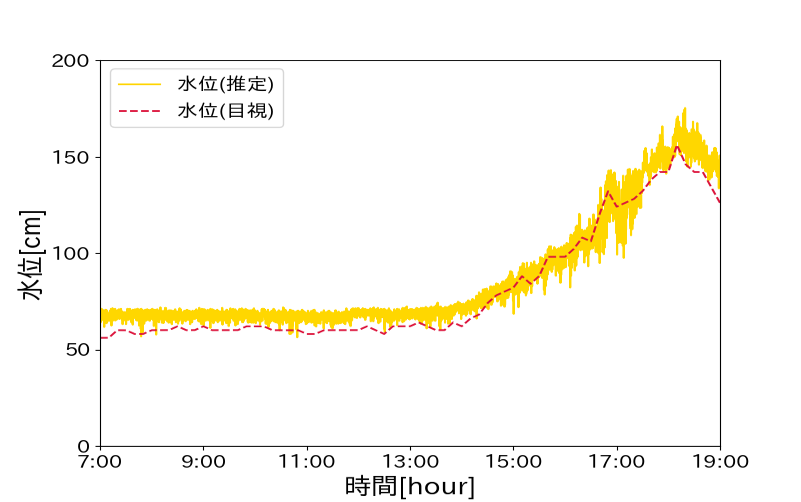
\includegraphics[width=\linewidth]{image/0706_ss.png}
  \end{center}
  \caption{SS手法の推定結果(テスト:7月6日)}
  \label{ss_0706}
\end{figure}


\begin{figure}[b] 
  \begin{center}
    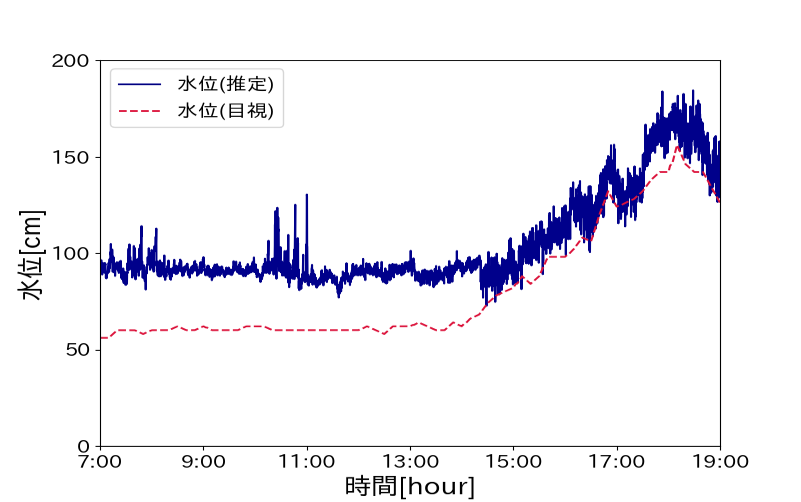
\includegraphics[width=\linewidth]{image/0706_senkou.png}
  \end{center}
  \caption{先行研究の手法の推定結果(テスト:7月6日)}
  \label{senkou_0706}
\end{figure}

\begin{figure}[h] 
  \begin{center}
    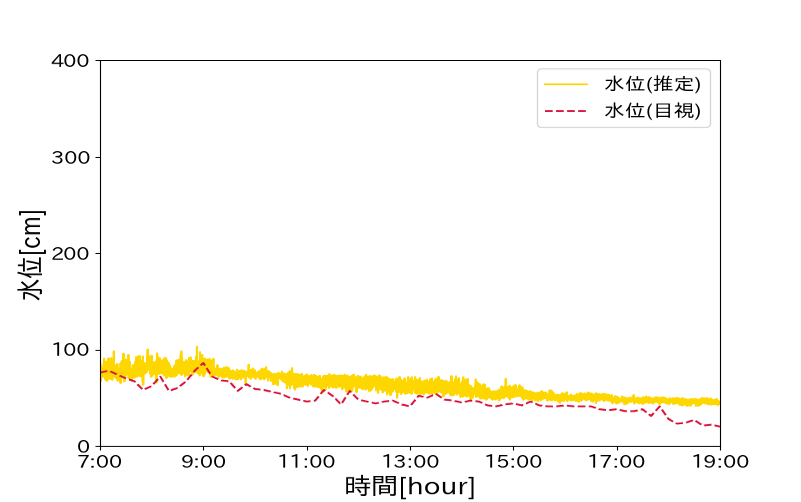
\includegraphics[width=\linewidth]{image/0707_ss.png}
  \end{center}
  \caption{SS手法の推定結果(テスト:7月7日)}
  \label{ss_0707}
\end{figure}

\begin{figure}[h] 
  \begin{center}
    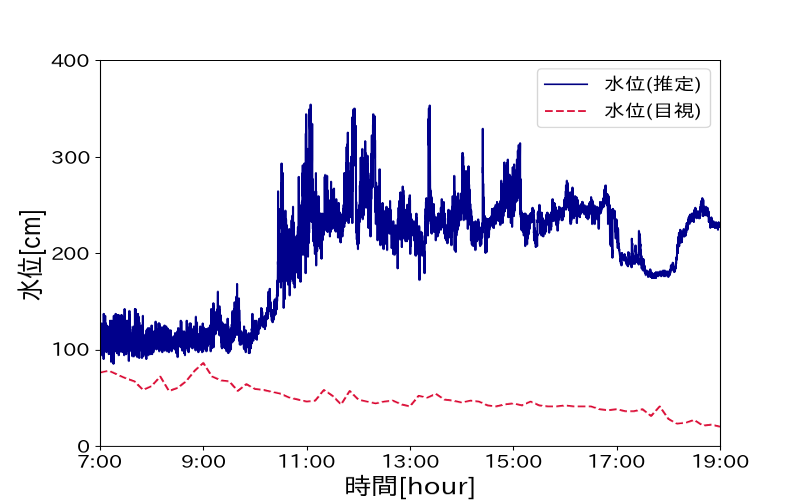
\includegraphics[width=\linewidth]{image/0707_senkou.png}
  \end{center}
  \caption{先行研究の手法の推定結果(テスト:7月7日)}
  \label{senkou_0707}
\end{figure}



\clearpage
\subsection{ラベル設定と評価}
\label{5.3}

水位計測ポールに対する
適切なラベル設定の調査を行うため,
アノテーション画像の水位計測ポールに対するラベル設定を変化させ,
モデルを作成し,推定した水位と目視で計測した水位とのRMSEと
IoUの比較を行った.設定Aと設定Bで作成した
アノテーション画像を使用して作成したモデル
で,水位の推定を行い,RMSEとIoUの比較を行う.
訓練データとテストデータには\ref{5.1}節と同じデータを使用し,
以下に設定Bの概要を示す.

\begin{description}
  \vspace{-3mm}
    \item ・水位計測ポールに水位計測ポールラベルを与える.
    \item ・水位計測ポール以外のラベル設定は設定Aと統一する.
\end{description}

それぞれの設定での,測定値とのRMSEとIoUは表\ref{pole}の通りとなった. 
また,それぞれの水位推定結果を図\ref{ss_0707}と図\ref{ss_pole}に,
時間別のIoUを図\ref{time_IoU_pole}に,
領域抽出例を図\ref{image_pole}に示す.

\begin{table}[ht]
  \centering
  \caption{RMSEとIoU}  
  \begin{tabular}{lrr} \bhline{1.5pt}
     &RMSE(cm)& IoU(%) \\ \hline 
   設定A&15.02&  92.30\\ \hline  
   設定B&15.66&  88.57\\ \hline  
  \end{tabular}
  \label{pole}
\end{table}

\begin{figure}[ht] 
  \begin{center}
    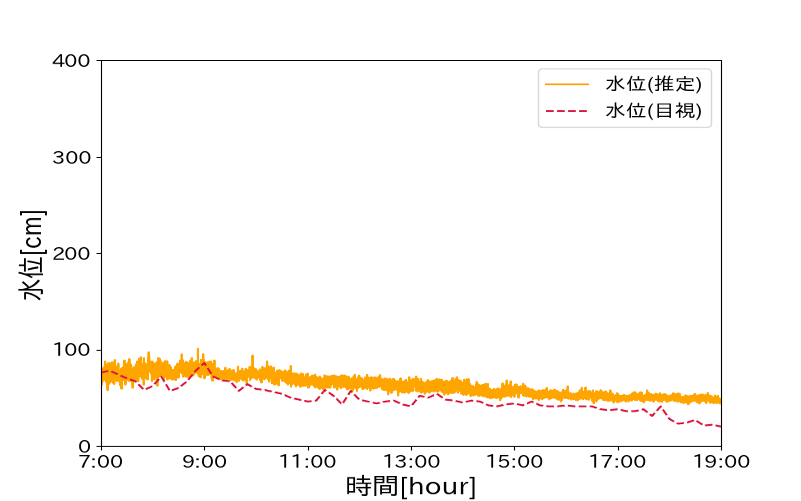
\includegraphics[width=\linewidth]{image/0707_ss_pole.png}
  \end{center}
  \caption{設定Bの推定結果}
  \label{ss_pole}
\end{figure}

\begin{figure}[ht] 
  \begin{center}
    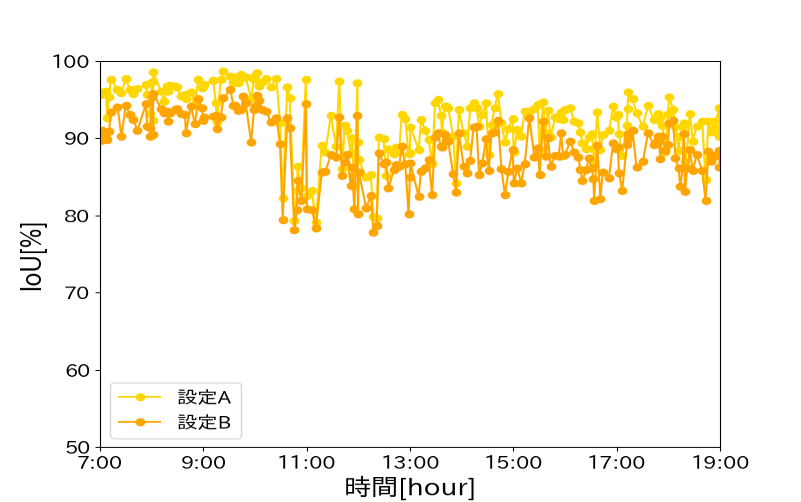
\includegraphics[width=\linewidth]{image/0707_IoU.png}
  \end{center}
  \caption{時間別IoU}
  \label{time_IoU_pole}
\end{figure}

\begin{figure}[t] 
  \begin{center}
    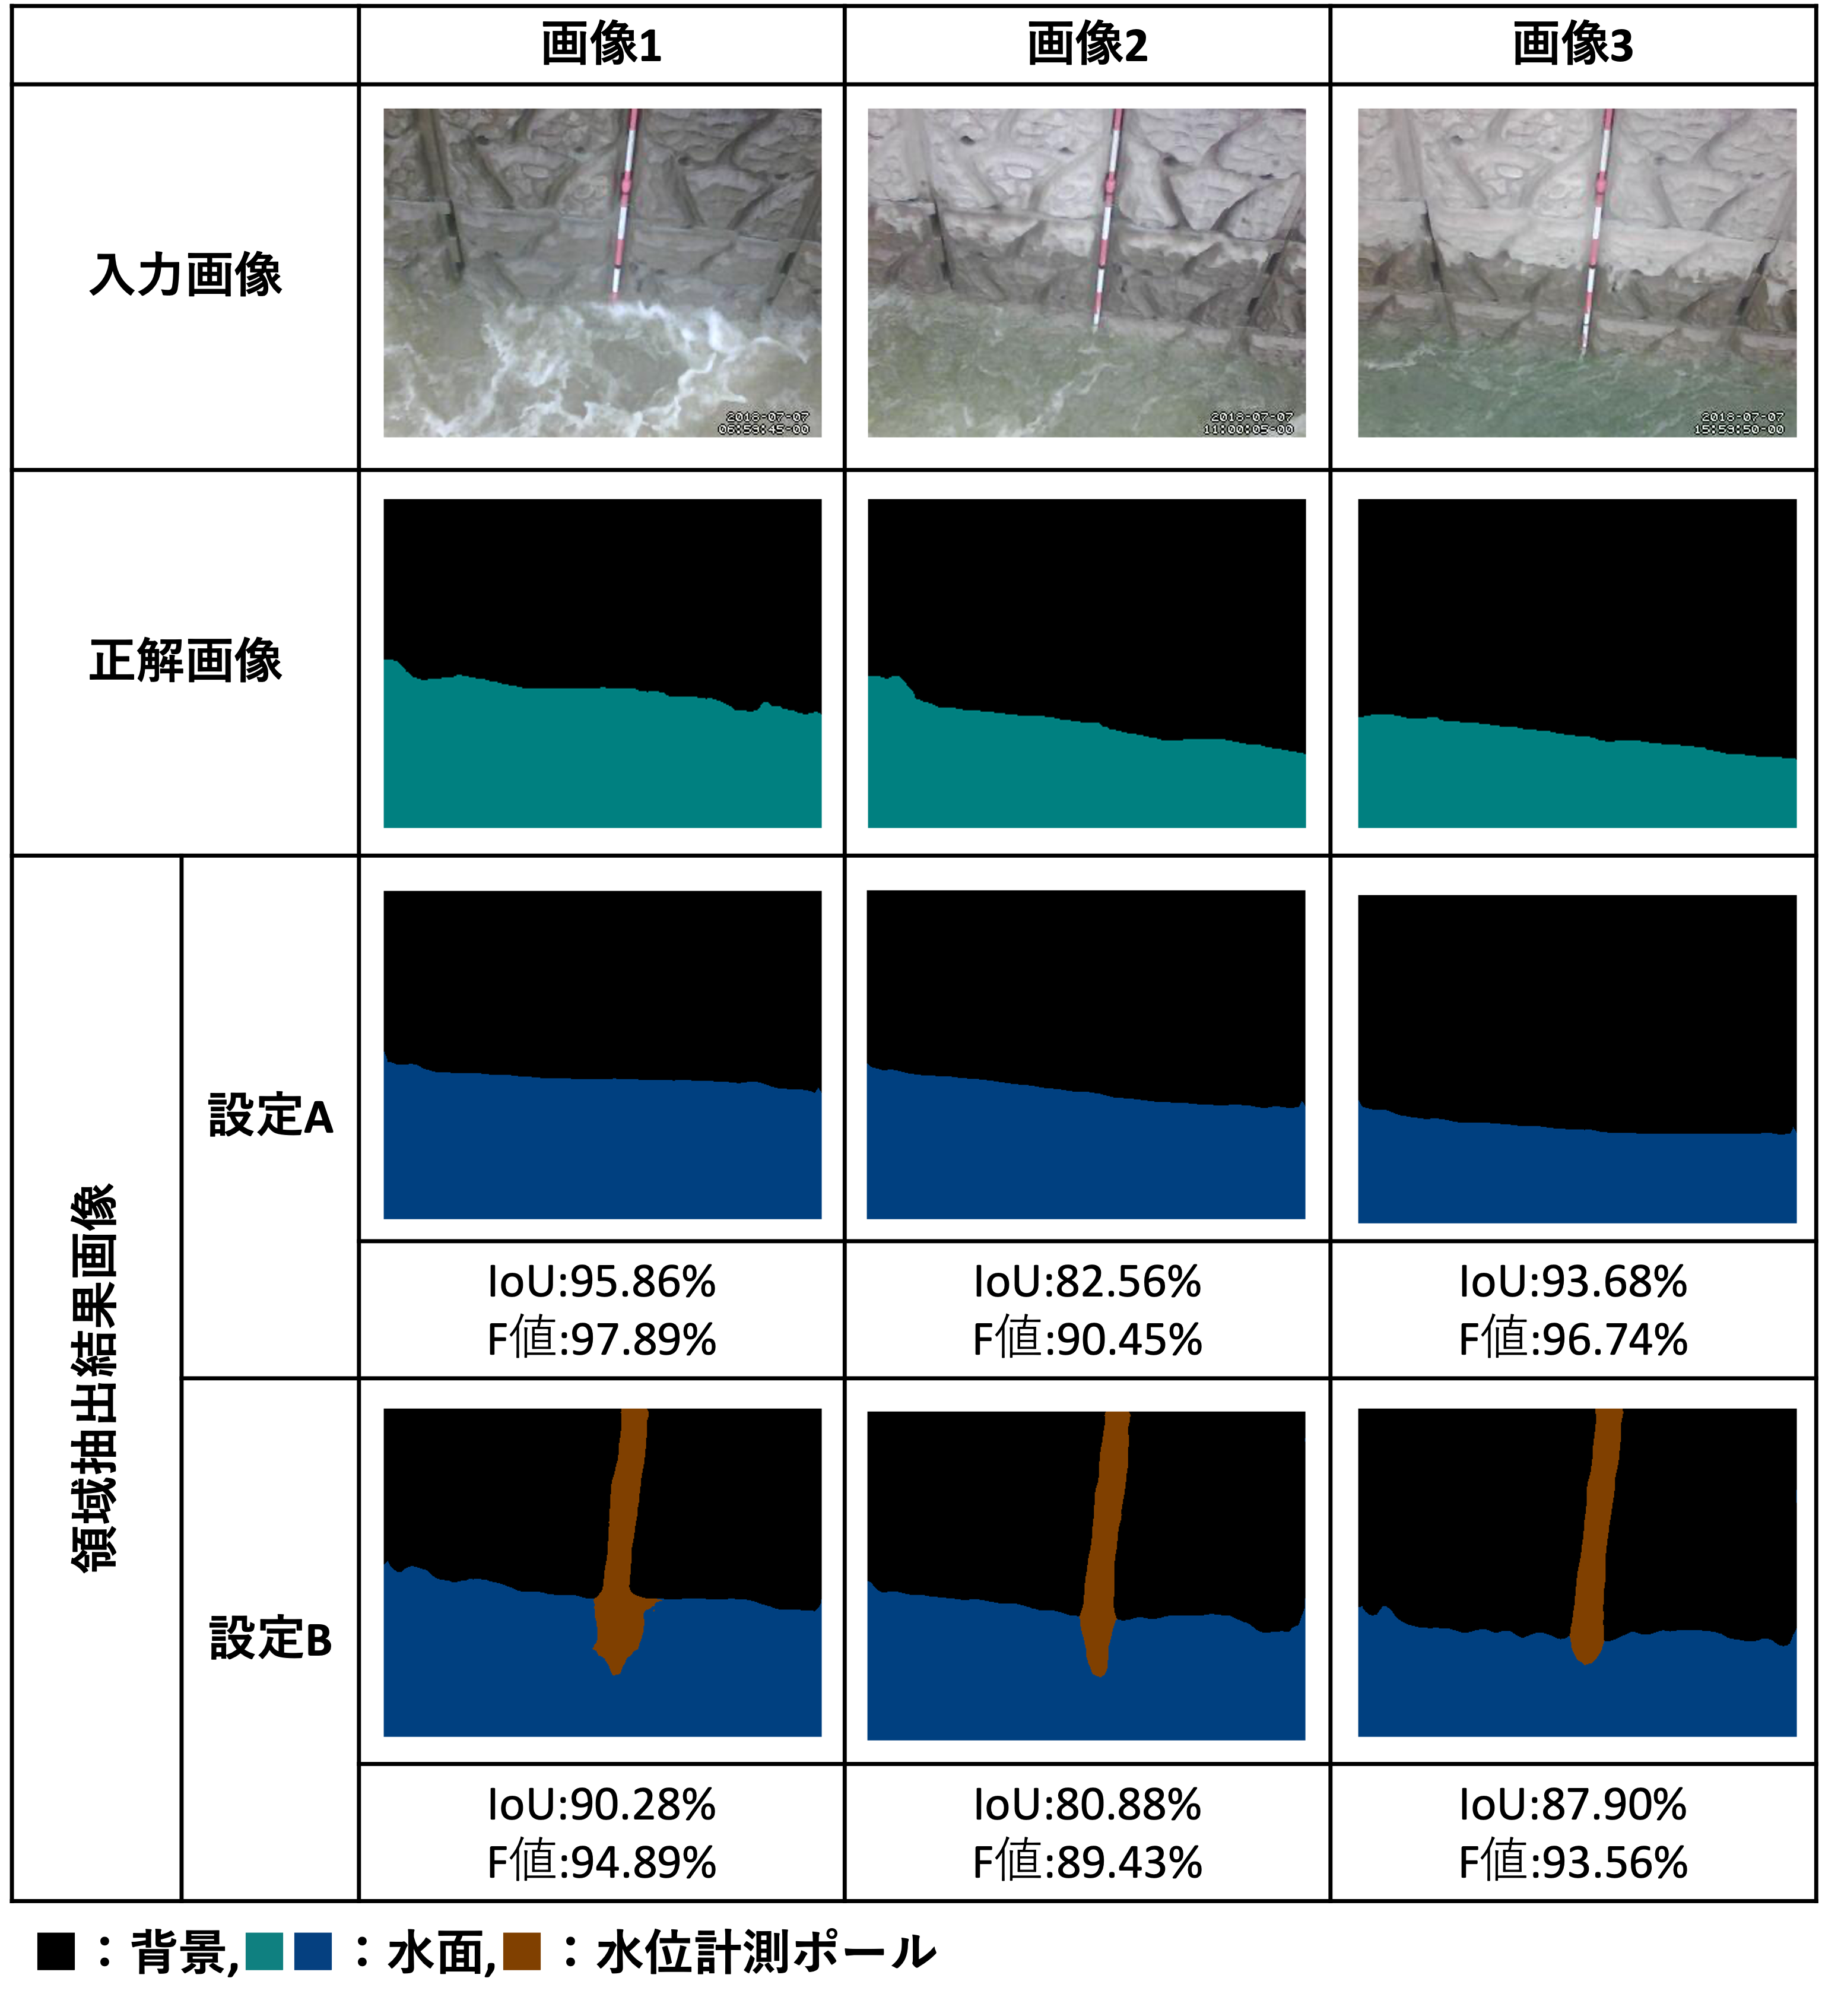
\includegraphics[width=\linewidth]{image/image_pole.png}
  \end{center}
  \caption{領域抽出結果例}
  \label{image_pole}
\end{figure}


\clearpage

\subsection{交差検証}
\label{5.4}
提案したアノテーション方法の評価するため,
2018年,7月5,6,7日の3日分の画像データを使用して交差検証(例:
7月5日と6日を訓練データ,7月7日をテストデータとして使用)を行った.
また,アノテーション設定は設定Aを使用した.

推定した水位と測定値とのRMSEとIoUは表\ref{kousa}の通りとなった. ま
た,それぞれの水位推定結果を図\ref{kousa_0705}から図\ref{kousa_0707}に,
時間別のIoUを図\ref{kousa_IoU_0705}から図\ref{kousa_IoU_0707}に,
領域抽出結果例を図\ref{images_kousa}に示す.
\begin{table}[ht]
  \centering
  \caption{RMSEとIoU}  
  \begin{tabular}{l|rrr} \bhline{1.5pt}
     &7月5日&7月6日&7月8日 \\ \hline 
   IoU(%)&88.33&  91.05&90.36\\ \hline  
   RMSE(cm)&17.32& 7.73&8.32\\ \hline  
  \end{tabular}
  \label{kousa}
\end{table}

\begin{figure}[ht] 
  \begin{center}
    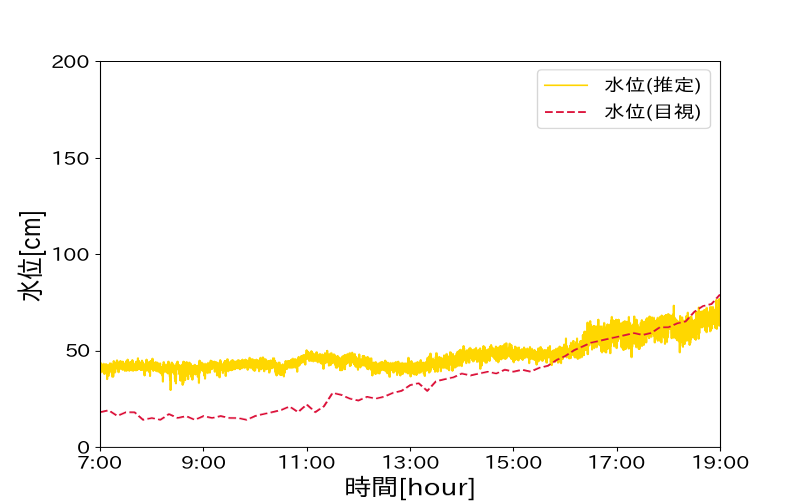
\includegraphics[width=\linewidth]{image/0705_kousa.png}
  \end{center}
  \caption{水位の推定結果(テスト:7月5日)}
  \label{kousa_0705}
\end{figure}

\begin{figure}[ht] 
  \begin{center}
    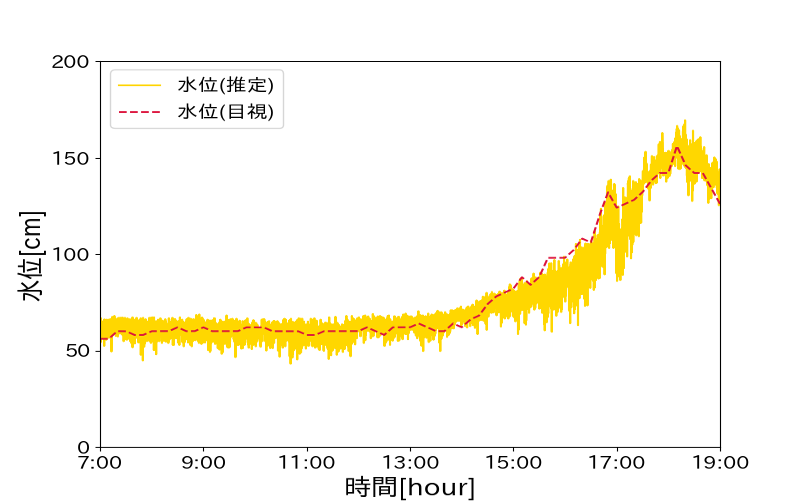
\includegraphics[width=\linewidth]{image/0706_kousa.png}
  \end{center}
  \caption{水位の推定結果(テスト:7月6日)}
  \label{kousa_0706}
\end{figure}

\begin{figure}[ht] 
  \begin{center}
    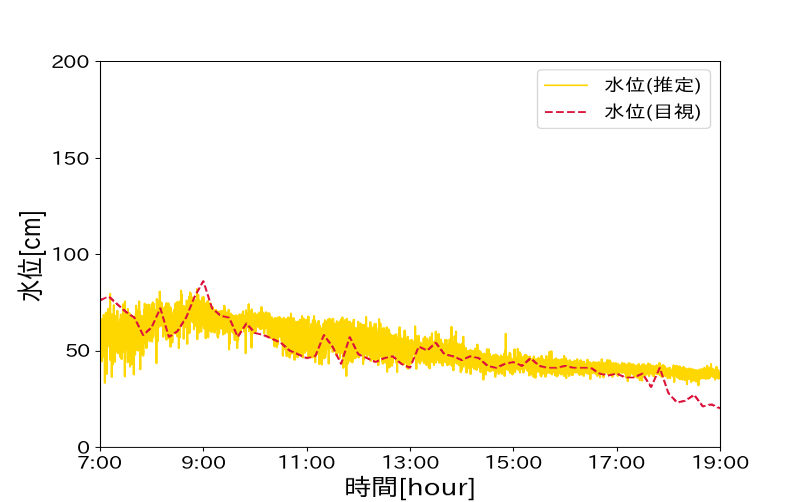
\includegraphics[width=\linewidth]{image/0707_kousa.png}
  \end{center}
  \caption{水位の推定結果(テスト:7月7日)}
  \label{kousa_0707}
\end{figure}

\begin{figure}[ht] 
  \begin{center}
    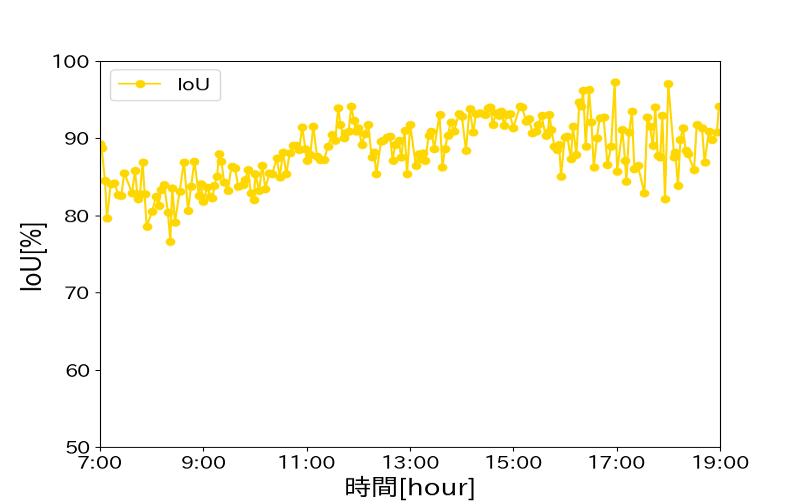
\includegraphics[width=\linewidth]{image/0705_IoU_kousa.png}
  \end{center}
  \caption{時間別IoU(テスト:7月5日)}
  \label{kousa_IoU_0705}
\end{figure}

\begin{figure}[ht] 
  \begin{center}
    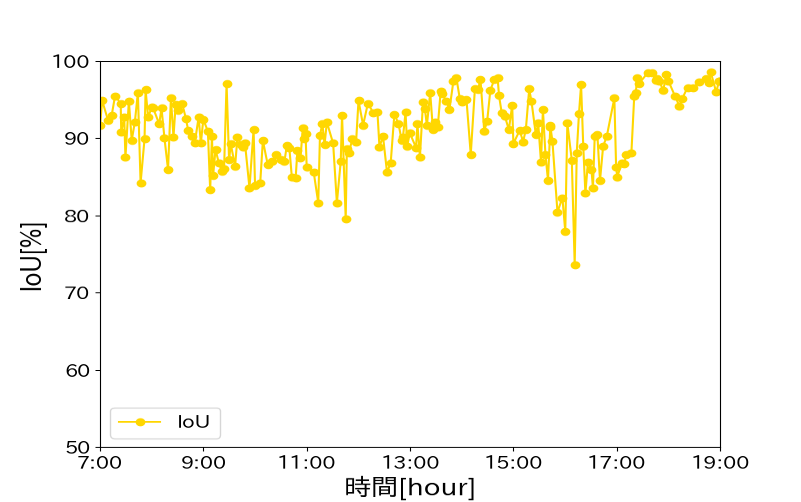
\includegraphics[width=\linewidth]{image/0706_IoU_kousa.png}
  \end{center}
  \caption{時間別IoU(テスト:7月6日)}
  \label{kousa_IoU_0706}
\end{figure}

\begin{figure}[ht] 
  \begin{center}
    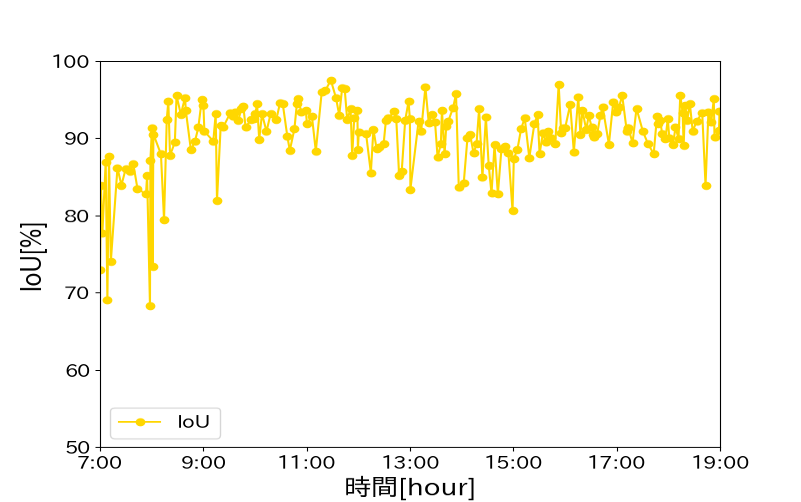
\includegraphics[width=\linewidth]{image/0707_IoU_kousa.png}
  \end{center}
  \caption{時間別IoU(テスト:7月7日)}
  \label{kousa_IoU_0707}
\end{figure}

\begin{figure}[t] 
  \begin{center}
    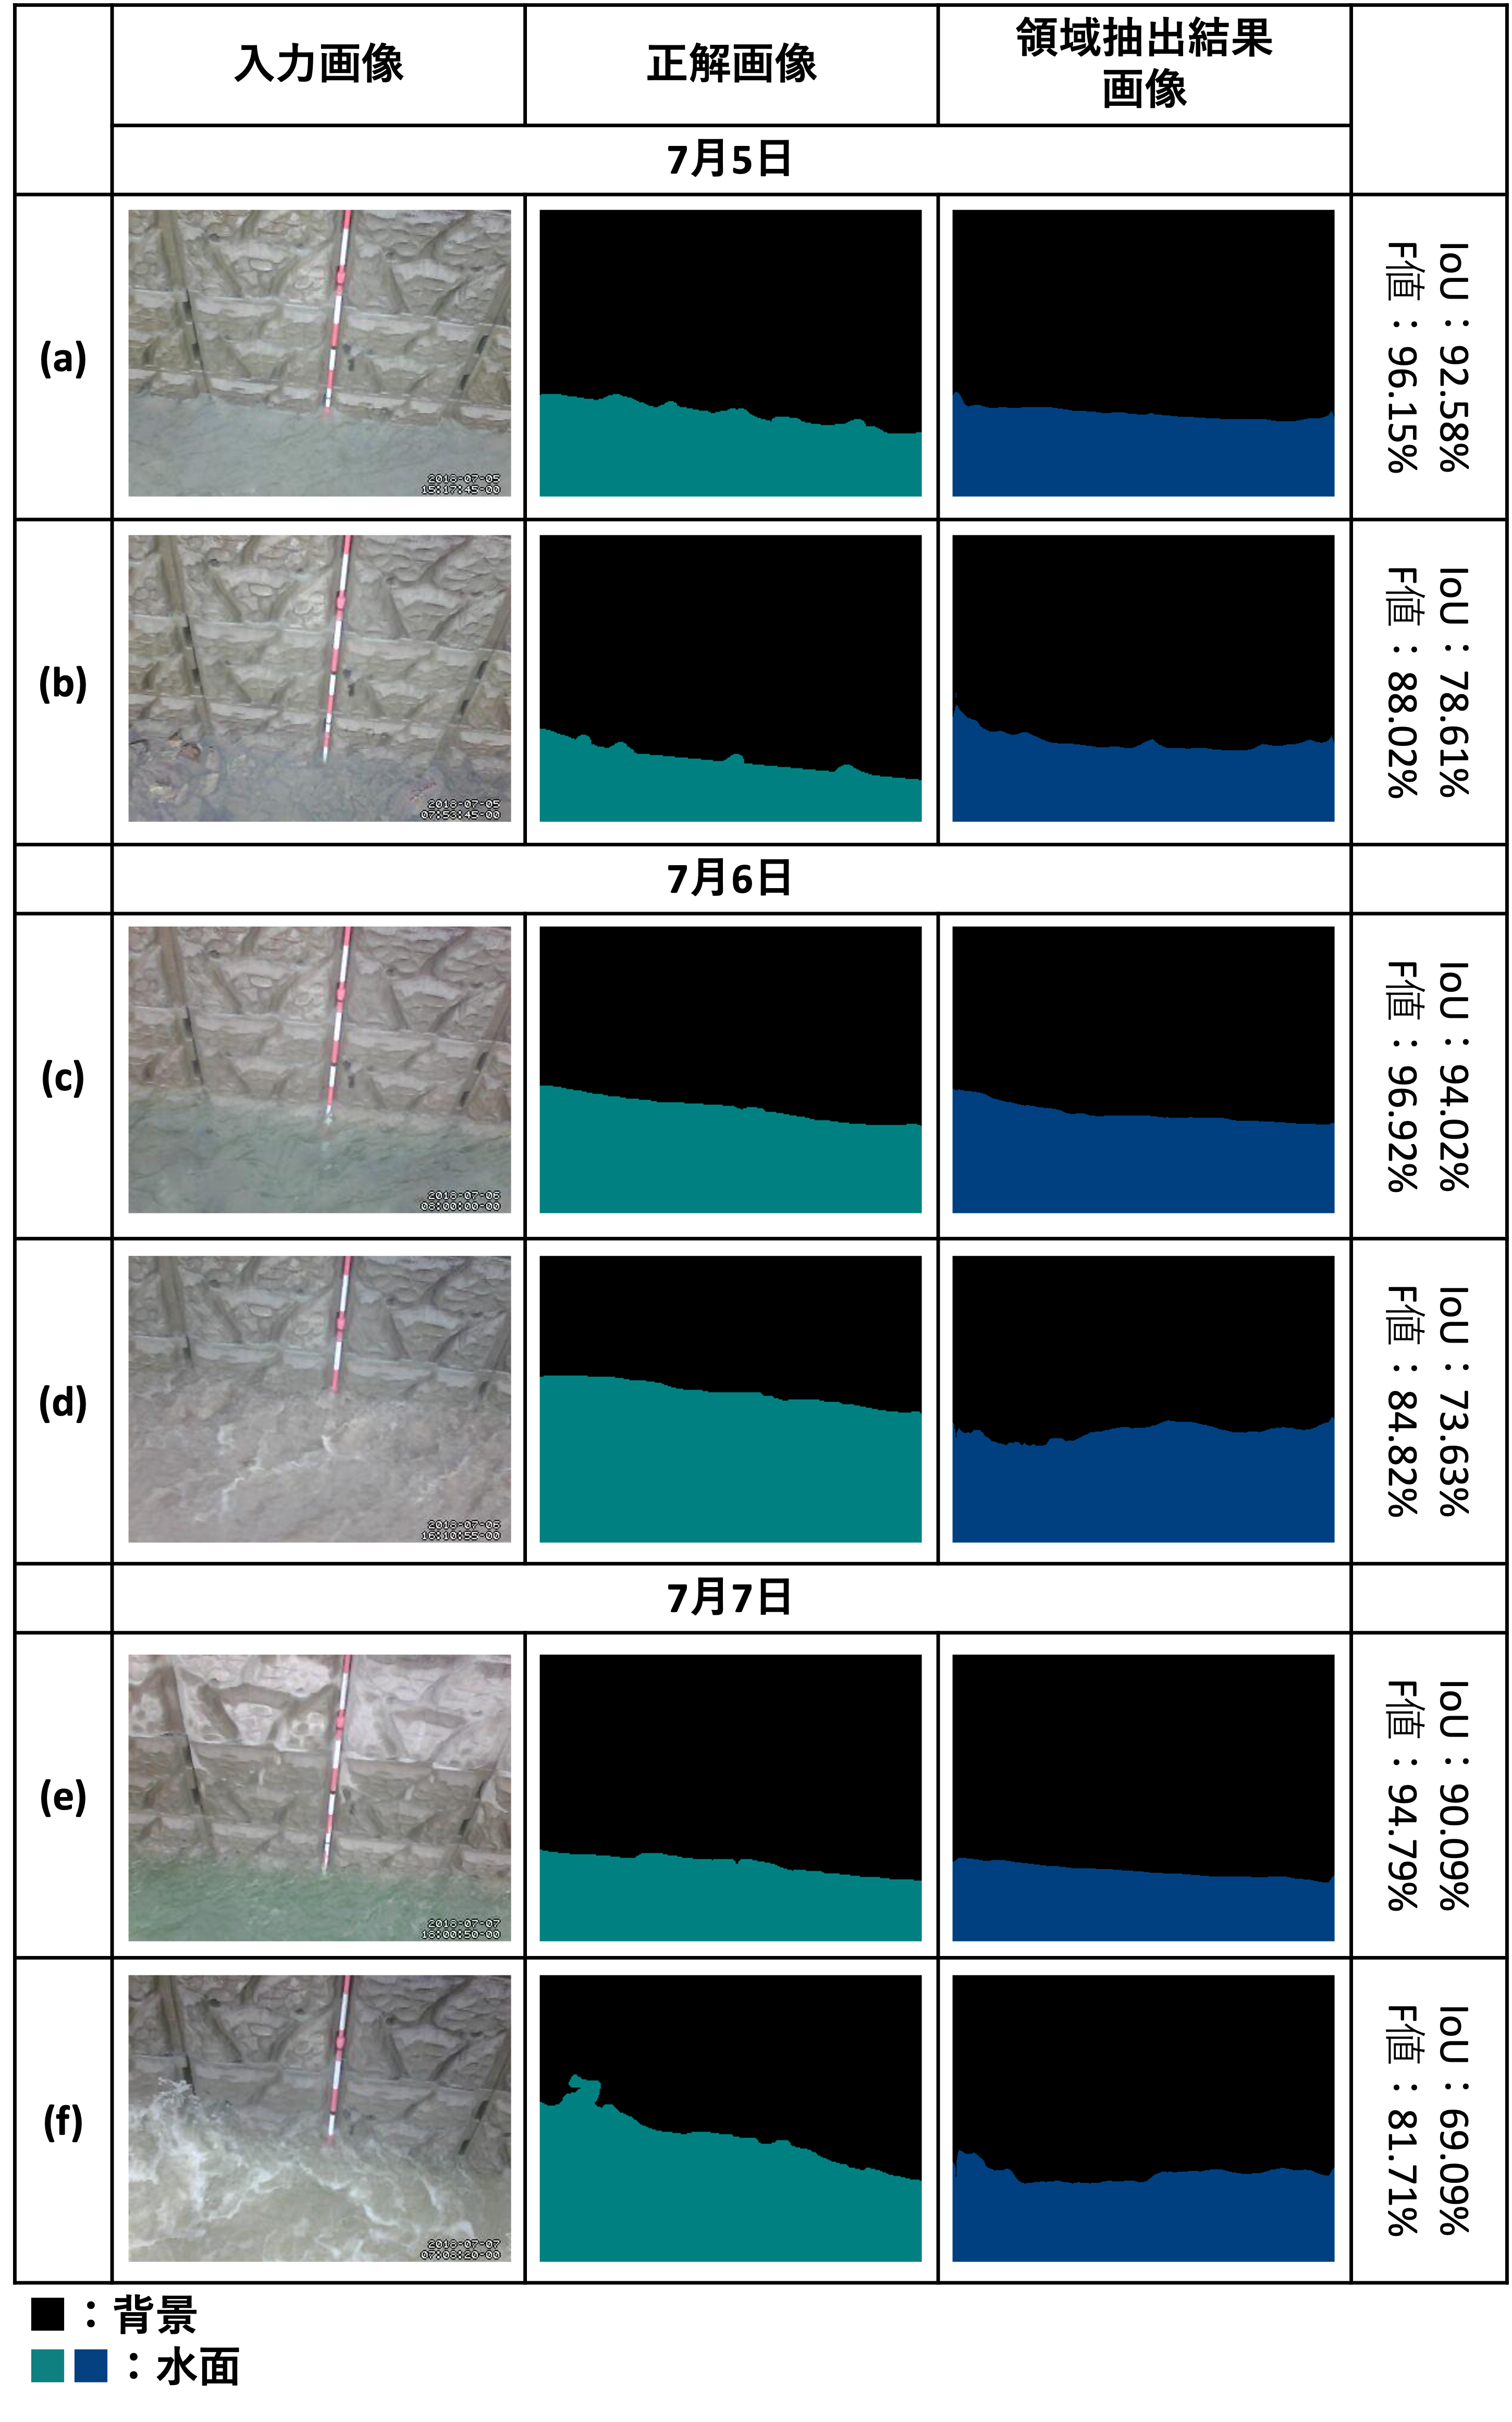
\includegraphics[width=120mm]{image/image_kousa.png}
  \end{center}
  \caption{領域抽出結果例}
  \label{images_kousa}
\end{figure}

%%%%%%%%%%%%%%%%%%%%%%%%%%%%%%%%%%%%%%%%%%%%%%
\clearpage
\section{考察}
\subsection{評価指標について}
IoU以外にもF score\cite{bf}という領域抽出結果の評価指標が存在する.
また,それは式(\ref{pr}),(\ref{re}),(\ref{fscore})と図\ref{tp}で表される.
F scoreは,トレードオフの関係であるPrecisionとRecallの両方の評価を行う.

\begin{center}
\begin{equation}
  \label{pr}
  \mbox{Precision} =  \frac{\mbox{TP}}{\mbox{TP}+\mbox{FP}}  
\end{equation}
\end{center}

\begin{center}
  \begin{equation}
    \label{re}
    \mbox{Recall} =  \frac{\mbox{TP}}{\mbox{TP}+\mbox{FN}} 
  \end{equation}
  \end{center}

\begin{center}
  \begin{equation}
    \label{fscore}
    \mbox{F score} =  2×\frac{\mbox{Precision}×\mbox{Recall}}{\mbox{Precision}+\mbox{Recall}}
  \end{equation}
\end{center}

以下に,F scoreとIoUは常に$\mbox{F score}≧\mbox{IoU}$という大小関係であり,以下にそれを示す.

\begin{align*}
  \mbox{F score}≧\mbox{IoU} &= \mbox{F score}-\mbox{IoU} ≧ 0    \\
          &= 2×\frac{\mbox{Precision}×\mbox{Recall}}{\mbox{Precision}+\mbox{Recall}}-\frac{\mbox{TP}}{(\mbox{TP}+\mbox{FP}+\mbox{FN})} \\
          &= \frac{2×\mbox{TP}}{(2\mbox{TP}+\mbox{FP}+\mbox{FN})}-\frac{\mbox{TP}}{(\mbox{TP}+\mbox{FP}+\mbox{FN})} \\
          &= \frac{\mbox{TP}(\mbox{FN}+\mbox{FP})}{(2\mbox{TP}+\mbox{FN}+\mbox{FP})(\mbox{TP}+\mbox{FP}+\mbox{FN})} \\
          &\mbox{TP},\mbox{FP},\mbox{FN}は正の整数より,\\
          &= \mbox{TP}\cdot(\mbox{FN}+\mbox{FP})≧0\\
          &同様に\\
          &= \mbox{TP}≧0 \\
\end{align*}
TPは正の整数であることから,常に$\mbox{F score}≧\mbox{IoU}$となる.また,IoUが0%,もしくは100%の時,
$\mbox{F score}=\mbox{IoU}$となる.以上より,F scoreとIoUの大小関係は変化しないため,
本研究では領域抽出結果の評価指標としてIoUを使用した.
\clearpage
\subsection{実験結果について}
5.1 節では,
セマンティックセグメンテーションモデルを
構築する最適な学習回数をモデルの領域抽出精度
から調査した.図\ref{kousa}より,200回からIoUは収束していることが確認できた.
したがって,モデルの学習回数は最低でも200回以上必要であるといえる.

5.2節では,SS手法を用いて推定した水位と目視で計測した水位とのRMSE
を先行研究の手法の結果と比較した.表\ref{kousa}より,SS手法を用いた場合 
の方がRMSEは小さくなった.先行研究の手法には,訓練に使用したデータと別の
データに対してテストを行うと精度が低くなるという問題があった.
しかし,SS手法のRMSEからSS手法は新規のデータに対しても
高精度で領域抽出ができていることが分かる.

5.3 節では,水位計測ポールに対する適切なラベル設定の調査を行った.
水位計測ポールの範囲に学習除外ラベルと水位計測ポールラベルを与え,作成したモデルのIoUとRMSEを比較した.
表\ref{kousa},図\ref{time_IoU_pole}より,学習除外ラベルを与えた場合の方がIoUもRMSEも
良い結果になることが確認できた.
図\ref{kousa}の領域抽出結果例から,
水位計測ポールに水位計測ポールラベルを与えた場合,
水面領域に覆いかぶさる形で水位計測ポールの推定を行っていることわかる.
このような推定により,IoUが低くなったと考えられる.
また,今回,水面領域面積の割合から水位の推定を行ったため,
水位計測ポール分水面領域面積が減少することにより,水位が少し低く推定されたと考えられる.

5.4節では交差検証を行い,提案したアノテーション方法の評価を行った.
提案手法を用いて作成したアノテーション画像を使用したモデルの
IoUはすべての日で,85%以上という結果になり,学習から除外した範囲があっても,
高精度の領域抽出が行えていることがわかる.
よって,提案したアノテーション方法の有効性を示すことができた.
しかし,他の日に比べて7月5日はIoUもRMSEも悪くなった.
特に,7月5日の7:00から12:00の範囲でIoUが低いことが図\ref{kousa_IoU_0705}より
確認できる.図\ref{images_kousa}より,7月5日の午前中は水位が低く,水面が澄んでいて,
肉眼でも水面と壁面の境界面を発見しにくくなっていることが影響したと考えられる.
また,7月6日は図\ref{kousa_IoU_0706}より,16:00から17:00の間で,7月7日は図\ref{kousa_IoU_0707}より7:00から9:00
の間で領域抽出精度が低い瞬間がある.
原因として図\ref{images_kousa}のように,河川の濁りが濃くなっていることが抽出に影響したと考えられる.


\clearpage
%%%%%%%%%%%%%%%%%%%%%%%%%%%%%%%%%%%%%%%%%%%%%%
\section{まとめ}
\label{7}
本研究では,深層学習を用いたセマンティックセグメン
テーションによって河川の監視カメラ画像から水位を推定することを目的とし,
訓練データとして必要なアノテーション画像を半自動的に作成する方法を提案した.
交差検証を行った結果,提案手法を用いて作成したモデルは全て
の日でIoUが85%以上となり,本手法の有効性が確認できた.
しかし,水面の状態によって精度が低くなるといった問題が見受けられた.
また,水位の推定方法としてSS手法を用いた手法を検討した.
SS手法と先行研究の手法を適用して推定した水位の誤差を比較した.
その結果,SS手法のRMSEが15.02cm,先行手法が163.44cmとなり,
SS手法の精度を確認したことで,SS手法の有効性を示せた.
今後の課題としては,他の河川に対する適用実験やアノテーション画像の自動生成などが
挙げられる.
\clearpage


%%%%%%%%%%%%%%%%%%%%%%%%%%%%%%%%%%%%%%%%%%%%%%

%%%%%%%%%%%%%%%%%%%%%%%%%%%%%%%%%%%%%%%%%%%%%%
%参考文献
\begin{thebibliography}{99}
  \bibitem{mlit}
  国土交通省:
  令和4年の土砂災害発生件数は795件,
  砂防NEWS Press Release,2023年3月

  \bibitem{zentyou}
  国土交通省水管理・国土保全局砂防部 : 
  「土砂災害警戒避難に関わる前兆現象情報の活用のあり方について」, 
  \url{http://www.mlit.go.jp/common/001021004.pdf}, 2006年3月. 

  \bibitem{seman}
  Nur Atirah Muhadi ,Ana Mijic , Ahmad Fikri Abdullah ,
  Siti Khairunniza Bejo , Muhammad Razif Mahadi: 
  Deep Learning Semantic Segmentation for Water Level Estimation Using Surveillance Camera, 
  , 2021年10月. 

  \bibitem{watanabe}
  渡邊 康平:
  土砂災害の前兆現象検知を目的とした画面分割と深層学習を用いた水位変動の推定,
  広島市立大学大学院情報科学研究科システム工学専攻修士論文,
  2023年1月. 

  \bibitem{deeplabv3+}
  Liang-Chieh Chen, Yukun Zhu, George Papandreou, Florian Schroff, Hartwig Adam: 
  Encoder-Decoder with Atrous SeparableConvolution for Semantic Image Segmentation, 
  , 2018年9月. 

  \bibitem{segnet}
  Vijay Badrinarayanan, Alex Kendall , and Roberto Cipolla, Senior Member: 
  SegNet: A Deep Convolutional Encoder-Decoder Architecture for Image Segmentation, 
  IEEE Transactions on Pattern Analysis and Machine Intelligence, 2017年12月. 

  \bibitem{IoU}
  青島 亘佐,山本 拓海,中野 聡,中村 秀明: 
  深層学習によるセグメンテーション手法を用いたコンクリート表面の変状領域の検出, 
  , 2020年7月. 
  
  \bibitem{bf}
  山根達郎,全邦釘,Tatsuro Yamane, Pang-jo Chun : 
  Deep learning による Semantic Segmentation を用いたコンクリート表面ひび割れの検出 , 
  構造工学論文集 Vol.65A, 2019年3月. 
  
\end{thebibliography}

